%Critique.tex
%Par Guillaume Lahaie
%LAHG04077707
%
%Critique du SRS Gestion de centre sportif fourni dans le cours. J'utilise un gabarit de tex pour l'écriture

%%%%%%%%%%%%%%%%%%%%%%%%%%%%%%%%%%%%%%%%%
% Simple Sectioned Essay Template
% LaTeX Template
%
% This template has been downloaded from:
% http://www.latextemplates.com
%
% Note:
% The \lipsum[#] commands throughout this template generate dummy text
% to fill the template out. These commands should all be removed when 
% writing essay content.
%
%%%%%%%%%%%%%%%%%%%%%%%%%%%%%%%%%%%%%%%%%

%----------------------------------------------------------------------------------------
%	PACKAGES AND OTHER DOCUMENT CONFIGURATIONS
%----------------------------------------------------------------------------------------

\documentclass[10.8pt]{article} % Default font size is 12pt, it can be changed here
\renewcommand{\familydefault}{\rmdefault}
\renewcommand{\thesubsection}{\alph{subsection}}

%Pour l'encodage avec accents
\usepackage[utf8]{inputenc}
\usepackage{longtable}
\usepackage{sidecap}

\usepackage{helvet}
\renewcommand{\familydefault}{\sfdefault}

\usepackage{afterpage}
\usepackage{appendix}
\usepackage{graphicx} % Required for including pictures
\usepackage{listings}

\usepackage[left=2.2cm,top=2.2cm,right=2.2cm,bottom=2.2cm,nohead]{geometry} % Required to change the page size to A4
\geometry{letterpaper} % Set the page size to be A4 as opposed to the default US Letter

\usepackage{float} % Allows putting an [H] in \begin{figure} to specify the exact location of the figure
\usepackage{wrapfig} % Allows in-line images such as the example fish picture


\linespread{1.15} % Line spacing

%\setlength\parindent{0pt} % Uncomment to remove all indentation from paragraphs

\graphicspath{{./Pictures/}} % Specifies the directory where pictures are stored
\usepackage[french,english]{babel}

%Comportement d'un paragraphe
\setlength{\parskip}{\baselineskip}%
\setlength{\parindent}{0pt}%

%Widows/orphans
\widowpenalty10000
\clubpenalty10000

\usepackage[hidelinks]{hyperref}

%Meta-info
\title{INF4500 - devoir 1}
\author{Guillaume Lahaie}
\date{Remise: 1er novembre 2013}

\hypersetup{
  pdftitle={INF4500 - devoir 1},
  pdfauthor={Guillaume Lahaie}
}

\newcommand\blankpage{%
  \null
  \thispagestyle{empty}%
  \addtocounter{page}{-1}%
  \newpage}

\begin{document}
\selectlanguage{french}

%----------------------------------------------------------------------------------------
%	TITLE PAGE
%----------------------------------------------------------------------------------------

\begin{titlepage}

\newcommand{\HRule}{\rule{\linewidth}{0.5mm}} % Defines a new command for the horizontal lines, change thickness here

\center % Center everything on the page

\textsc{\LARGE Université du Québec à Montréal}\\[1.5cm] % Name of your university/college
\textsc{\Large INF4500}\\[0.5cm] % Major heading such as course name

\HRule \\[1.5cm]
{ \huge \bfseries Devoir 1}\\[0.4cm] % Title of your document
\HRule \\[1.5cm]

\begin{minipage}{0.4\textwidth}
\begin{flushleft} \large
\emph{Par:}\\
Guillaume Lahaie \\ LAHG04077707 % Your name
\end{flushleft}
\end{minipage}
~
\begin{minipage}{0.4\textwidth}
\begin{flushright} \large
\emph{Remis à:} \\
Abdoulaye Baniré Diallo % Supervisor's Name
\end{flushright}
\end{minipage}\\[4cm]

{\large \emph{Date de remise:} \\ Le 1\textsuperscript{er} novembre 2013}\\[3cm] % Date, change the \today to a set date if you want to be precise

%\includegraphics{Logo}\\[1cm] % Include a department/university logo - this will require the graphicx package

\vfill % Fill the rest of the page with whitespace

\end{titlepage}
\blankpage

%----------------------------------------------------------------------------------------
%	TABLE OF CONTENTS
%----------------------------------------------------------------------------------------

\tableofcontents % Include a table of contents

\newpage % Begins the essay on a new page instead of on the same page as the table of contents 

%----------------------------------------------------------------------------------------
% SECTIONS DU DOCUMENT
%----------------------------------------------------------------------------------------
%TODO: vérifier si mes orientations sont corrects.
%TODO: Vérifier le lien entre les gènes portant les noms ALS2CR...
\section{Question 1} % Major section

\subsection[Description du gène ALS2]{Description sommaire du locus du gène ALS2 chez l'Homo sapiens.}

J'ai consulté deux sources pour obtenir des informations sur la location du gène ALS2 (\emph{amyotrophic lateral sclerosis 2 (juvenile)}) de l'humain. La première source,
afin d'identifier la location du locus, était le UCSC genome browser. La recherche a été effectuée sur la version GRCh37/hg19
du génome humain. Comme on peut le voir sur l'image en annexe \ref{1}, le gène ALS2 est sur le brin q, c'est-à-dire qu'il est sur le brin complémentaire, donc il est orienté 3` $\rightarrow$ 5`.

Le locus du gène est situé sur le chromosome, à la position 2q33.1. La position précise du gène est chr2:202,564,986-202,645,895.
Sa taille est donc 80 910 pairs de nucléotides. J'ai effectué la même recherche ensuite dans la base de données du
\emph{National Center for Biotechnology Information} (NCBI). J'ai effectué une recherche dans la base de données des gènes,
j'insère en annexe \ref{2}  une image de la région du chromosome 2 où se situe le gène. On retrouve les mêmes informations
à propos du gène ALS2: la location, la taille et sa location précise sont les mêmes que UCSC. Afin de trouver la distribution
des nucléotides dans le gène, j'ai écrit un script biopython (annexe \ref{3}) prenant en entré le fichier genbank de la séquence
du gène et retournant la distribution. Le résultat de cette analyse est détaillé à la table \ref{tab:first}.
\begin{table}[b]
{\small
\centering
\begin{tabular}{|c|c|c|}

 \hline
 Nucléotides & Compte & Pourcentage \\
 \hline
 A & 23361 & 28.87\% \\
 \hline
  C & 15070 & 18.62\% \\
 \hline
  G & 15717 & 19.43\% \\
 \hline
  T & 26762 & 33.08\% \\
 \hline
  Total & 80910 & 100\% \\
 \hline
 \end{tabular}
\caption{{\small Distribution des nucléotides dans le locus du gène ALS2}}
\label{tab:first}
}
\end{table}

NCBI donne un sommaire du rôle du gène ALS2. Il encode une protéine, et son nom est donné dans le fichier genbank de la séquence
nuclétidique: l'alsin. Afin d'avoir une meilleure idée de la fonction du gène ALS2, j'ai effectué une recherche sur 
\emph{Genetics Home Reference} (GHR). La protéine semble avoir plusieurs rôles, entre autres l'activation de 
protéines de la famille des GTPases, qui joue un rôle important dans la division cellulaire, la différentiation. Ce gène semble surtout
connu pour son lien à la Sclérose latérale amyotropique, aussi connue sous le nom de la maladie de Lou Gherig. 
Toutefois, seulement 5 à 10\% des cas de cette maladie serait de cause génétique. %TODO SOURCE

\subsection[Loci voisins du gène ALS2]{Comparaision des loci voisins au gène ALS2.}

J'ai tout d'abord suivi le lien \emph{Map Viewer} de la description du gène ALS2 pour trouver la location 
du gène ALS2 (annexe \ref{4}).  Cette vue permet d'identifer deux loci voisins immédiats, les loci des gènes 
MPP4 et RPS2P16. J'ai ensuite passé changé les valeurs des nucléotides de début et de fin afin de voir la
séquence 202M - 203M du chromosome 2 de l'humain (annexe \ref{5}). Cette vue permet de d'observer plusieurs autres
loci de gènes. J'ai choisi de décrire les loci des gènes MPP4, RPS2P16, CDK15, TMEM237 et ENO1P4.

On peut séparer ces gènes en deux catégories. La première catégorie sont des pseudogènes. En effet,
Selon la description des gènes RPS2P16 et ENO1P4, il s'agit de deux pseudogènes, c'est-à-dire des
gènes qui ne sont plus exprimés chez l'humain. Ils ont donc un rôle différent du gène ALS2. Ils ont toutefois
une relation avec ce gène car ils sont situés à la même location du chromosome 2. Le gène RPS2P16 
(\emph{ribosomal protein S2 pseudogene 16}) est situé à la location 2q33.1 du chromosome 2, et il 
est orienté 5' $\rightarrow$ 3'. Plus précisément, il occupe la séquence 202627437 - 202628333 du 
chromosome 2, et a une taille de 896 bp. Le gène ENO1P4 (\emph{enolase 1, (alpha) pseudogene 4})
est situé  à la location 2q33.1, plus précisément la séquence 202486369 à 202488153 de la séquence de référence
du chromosome 2 de l'humain. Il a donc une taille de 1784bp. Il a une orientation 3' $\rightarrow$ 5'. 

La deuxième catégorie de gènes est plus similaires à ALS2. En effet, les gènes MPP4 
(\emph{membrane protein, palmitoylated 4 (MAGUK p55 subfamily 4)}), CDK15 (\emph{cyclin-dependant kinase 15}) et
TMEM237 (\emph{transmembrane protein 237}) sont tous des gènes qui encodent une protéine. On remarque
aussi que dans les noms synonymes, ils ont un nom similaire à ALS2. Le nom ALS2CR5 pour MPP4, ALS2CR7 pour CDK15 et
ALS2CR4 pour TMEM237, alors que le gènes ALS2 est aussi connu sous le nom ALS2CR6. Toutefois une recherche pour
identifier ce lien n'a pas permis de découvrir un lien précis, cela semble lié à la région du chromosome.

Les fonctions possibles de ces trois gènes semblent différentes de la fonction de ALS2. Le gène MPP4, situé à la
la position 2q33.2, il est donc lui aussi sur le brin 3' $\rightarrow$ 5'. Le gène a une taille de 53 821bp. Il 
produit une protéine membre de la famille MAGUK, qui se retrouve surtout dans la rétine. Le gène CDK15 est situé
à la location 2q33.2, plus précisément à la séquence 202655177 - 202760273 du chromosome 2, il a donc une taille 
de 105 096 bp. Il est sur le brin complémentaire, dans la direction 5' $\rightarrow$ 3'. Il serait impliqué 
dans le contrôle du cycle "eucaryotique" des cellules. Finalement, le gène TMEM237 est situé à la location 2q33.2,
donc sur le brin complémentaire, plus précisément à la séquence 202484907 - 202508252 du chromosome 2. Il a donc
une taille de 23345 bp. La protéine encodée par ce gène semble être impliqué dans "WNT signaling" (refseq 2012). 

\subsection[Annotations du gène ALS2]{Description des annotations du locus du gène ALS2.}

Afin de décrire les annotations du locus du gène ALS2, Je prendrai la vue de MapViewer en annexe \ref{3}. La première annotation, 
donnant des informations du gène, a déjà été décrite en a. La prochaine annotation, celle des OMIM, nous propose quatre résultats. 
Trois des résultats sont des maladies génétiques reliées au gène ALS2. La première est \emph{Primal Lateral Sclerosis Juvenile} (PLSJ),
une maladie se rapprochant de ALS, mais qui est généralement moins sévère. La seconde maladie est la sclérose amyotrophique latérale, 
que nous avons déjà décrite, et la dernière maladie est \emph{Spastic paralysis, infantile-onset, ascending} (IAHSP). 
Ces trois maladies ont un lien avec une mutation du gène ALS2. Le dernier résultat de la recherche OMIM présente des informations à
propos de l'alsin, la protéine encodée par le gène ALS2. Selon Yang et al. et Hadano et al., ce gène comporte 34 exons 
dans une région de 83kb.

La prochaine annotation envoie vers HGNC, un annuaire de liens utiles à propos de ALS2. L'annotion suivante (sv) 
est un lien vers sequence viewer, une représentation graphique de la séquence nucléotidique du gène. On peut ainsi voir graphiquement la
position des features du fichier, par exemple les STS, les CDS. Ensuite, l'annotation pr montre les résutlats de la recherche dans la
banque de données des protéines de la protéine encodée par ce gène. On y retrouve 19 résultats, la majorité reliée à la protéine alsin,
qui est encodée par ALS2. 

L'annotation dl permet d'obtenir un fichier contenant la séquence nucléotidique exacte du gène.
Il est possible d'obtenir le fichier en format fasta ou genbank. Selon la prochaine annotation (ev), on peut retrouver
37 exons et 2 gènes dans la séquence de 81 710bp du gène ALS2, Ce résultat provient de l'alignement de 12 modèles. 
La prochaine annotation (hm) nous donne l'ensemble des gènes homologues au gène ALS2, nous reviendrons sur cette annotation au point e. 
Finalement, l'annotation sts nous permet de trouver les 9 STS contenus dans le locus du gène ALS2. 
On remarque ici qu'on obtient un nombre différent de STS que dans l'annotation sv.

\subsection[Fichier genbank du gène ALS2]{Analyse du fichier genbank du locus du gène ALS2.}

Afin de trouver le fichier genbank associé au locus du gène ALS2, je prends le lien vers le fichier genbank situé dans la section
\emph{Genomic regions, transcripts, and products} de la page du gène. Le fichier genbank obtenu représente une région plus
grande que celle du gène ALS2, donc j'ai cherché la "feature" du gène ALS2 particulièrement.

Regardons tout d'abord les informations générales du fichier.La première ligne nous donne quelques informations de base: le numéro
d'accession (NC\_000002), le nombre de pairs de nucléotides dans le fichier (80 910 bp), que la séquence représentée est une séquence
d'ADN, que cet ADN est linéaire et que la dernière modification date du 13 août 2013. On voit ensuite que cette séquence apparait 
dans le génome de l'humain, et qu'elle est situé sur la région complémentaire du chromsome 2, et qu'il s'agit de la version 11 de la
séquence.

La feature du gène ALS2 nous indique que la région de ce gène se situe dans la sous-séquence 12136 à  93045 de la séquence. On y 
remarque quatre variantes de la transcription en ARN messager, et donc quatree CDS particuliers pour ces variantes.
Chacune de ces variantes a comme note que le gène est dérivé d'une analyse automatisée, les résultats de forme X1 et X2 ont été
obtenue à partir de la méthode Gnomon, tandis que les résultats de forme 1 et 2 ont été obtenues à partir de la méthode
bestrefseq. On indique pour chaque région les synonymes du gène ALS2, qui sont ALS2CR6, ALSJ, IAHSP et PLSJ. Chaque feature CDS
du gène ALS2 indique le codon de début de la transcription, qui est le codon 1 pour les quatre variantes. On indique aussi la
protéine encodée, qui est une forme de la protéine alsin pour les quatre CDS. Finalement poru chaque CDS, on indique la
chaine d'acide aminée obtenue suite à la transcrition. Comme il y a plusieurs formes les transcriptions sont différentes.

Ce fichier genbank ne comprend pas les annotations STS, alors pour vérifier ces propriétés, j'ai effectué une recherche dans la
base de données de nucléotides de ncbi pour trouver un contig contenant plus d'informations. J'ai trouvé le fichier ayant le
numéro d'accession NG\_008775.1, qui contient une information plus complète. Ce fichier ne comprend qu'une seule annotation mRNA
et CDS pour le gène ALS2, on y retrouve toutefois la position de tous les exons du gène, ainsi que les STS. Ce locus contient
9 STS, et 34 exons pour le gène ALS2. 

\subsection[Homologues du gène ALS2]{Homologues du gène ALS2.}

Afin de vérifier si ce gène a des homologues, j'ai consulté l'annotation \emph{hm} de Map Viewer pour le gène ALS2. (Il aurait
été aussi possible de faire une recherche blast pour trouver le résultat.) On retrouve un homologue de ALS2 chez les espèces suivantes:
le chimpazé (Pan troglodytes), le macaque rhésus (Macaca mulatta), le chien (Canis lupus familiaris), le boeuf (Bos taurus), la souris
(Mus musculus), le rat de Norvège (Rattus norvegicus), le poulet (Gallus gallus) et le poisson zèbre (Danio rerio). 

En regardant le fichier du gène homologue, on ne retrouve pas d'information sur le rôle que ce gène occupe
chez l'espèce. On peut toutefois regarder la protéine obtenue pour tenter de répondre à la question du rôle joué.
On remarque que ce gène produit une forme de la protéine alsin chez tous les homologues. De plus, on peut aussi remarqué
que le nombre d'acides aminées des protéines obtenues est très similaires: il varie de 1649 à 1681 acides aminées. Il semble
donc que ces protéines jouent des rôles similaires chez ces espèces, mais il faut obtenir plus de données à ce sujet pour être 
certains que les rôles sont similaires.

%----------------------------------------------------------------------------------------
% SECTIONS DU DOCUMENT
%----------------------------------------------------------------------------------------
 
\section{Question 2} % Major section

Utilisez le programme CAP3 pour assembler les reads du SARS. Vous obtiendrez comme résultat plusieurs contigs. Concentrez
votre analyse sur cinq contigs que vous choisirez.

\subsection[Qualité des contigs]{Que pouvez-vous dire de la qualité des contigs?}

Afin de créer les contigs à partir des reads, j'ai utilisé la version de CAP3 disponible sur le serveur Mobyle@Pasteur.
L'application a produite 216 contigs à partir des données. J'ai ensuite écrit un script byopython (annexe \ref{7}) permettant de choisir
au hasard 5 contigs et d'effectuer un blast sur ces contigs. Le script a choisi au hasard (à l'aide d'un générateur de
nombres pseudoaléatoires) les contigs 7, 132, 195, 209 et 214.

Avant d'analyser les résultats du blast, regardons tout d'abord la qualité de ces contigs. Pour le contig 7 (résultat annexe \ref{8}),
la grande majorité des valeurs est 25, avec quelques endroits ayant une valeur de 10, et à certains endroits des 5 ou des 0.
Ces valeurs sont basées sur l'échelle Phred, qui est un score ayant une relation logarithmique. Avec une valeur de 25, 
la probabilité d'une identification incorrecte se situe à plus de 99\%, alors qu'une valeur de 10 indique qu'il y a 90\% de chance
d'un bon choix . Il semble donc que le contig est de bonne qualité, avec quelques endroits où la qualité est plus basse. Ces endroits
se situent surtout au début et à fin du contig.

Le résultat de qualité du contig 132 (annexe \ref{9}) est plus bas que le précédent. La majorité du contig a une valeur de qualité
de 20, et il y a une séquence d'environs 400 nucléotides à la fin du contig ayant une qualité variant de 0 à 15, ainsi qu'une séquence
d'environ 80 nucléotides au début ayant une qualité de 10 ou 15. Le résultat est quand même généralement acceptable, avec une moyenne de
99\% de précision, sauf aux extrémités, où le résultat a environ 90\% de précision.

Le contig 195 (résultat de qualité annexe \ref{10}) a une qualité assez faible. La première moitié du contig a un score de
qualité de 15 en moyenne, alors que la seconde moitié a un score de 10, avec une très petite séquence au milieu du contig
ayant un résultat de 20 ou plus. Ce contig a donc un résultat de précision beaucoup plus que les deux autres contigs choisis.

Le contig 209 (résultat de qualité annexe \ref{11})a un résultat de qualité similaire au contig 7. Les scores des nucléotides 
sont majoritairement 25, avec une séquence à la fin ayant un score plus faible, entre 10 et 15. La précision pour ce contig est
donc très haute.

Finalement, le contig 214 (résultat de qualité annexe \ref{12}) a une très grande variation de qualité. On retrouve au milieu
de contig une qualité très élevé, avec certaines séquences ayant un score de qualité de 30 ou même 35. Toutefois, le début et
la fin du contig souffre d'une qualité beaucoup plus basse, avec une séquence ayant un score de 0, et une séquence ayant un score
de 10 à la fin du contig.

\subsection[Blast des contigs]{Blastez vos contigs}

Les 5 contigs choisis ont été blastés avec le script biopython en annexe \ref{7}. Les résultats ont été enregistés dans des
fichiers en format xml. Afin d'obtenir une interprétation graphique des résultats, j'ai aussi effectué le blast à partir de
l'interface web de NCBI. Pour les deux séries de blast, j'ai choisi comme option de blaster contre la base de données nr, 
et d'utiliser blastn, c'est-à-dire de rechercher des séquences assez similaire.

Le résultat graphique des 5 contigs est disponible à l'annexe \ref{13}. Au premier regard, on remarque que tous les résultats
sont à peu près pareils. Un regard rapide aux fichiers xml confirment ce fait. Tous les résultats ont le même total score,
environ la même longueur de hit, et ont tous une e-value de 0.

\subsection[Fonctions prédites des contigs]{Quelles sont les fonctions prédites par les différents contigs choisis?}

Pour essayer de prédire les fonctions, je vais regarder les informations des fichiers genbank des dix premiers résultats
blast de chaque contig choisi. Pour ce faire, j'utilise le script en annexe \ref{14}.

Quatre des contigs choisis semblent avoir une fonction commune. En effet, pour les contigs 7, 196, 209 et 214, on retrouve
des annotations semblables dans les fichiers genbank obtenus des résultats des blast. On y retrouve des annotations pour deux
gènes et deux CDS encodant les protéines suivantes: \emph{orf1ab polyprotein} ou \emph{polyprotein orf1ab} (PP1ab), ou encore
\emph{orf1a polyprotein} ou \emph{polyprotein orf1a} (PP1a). Les fichiers genbank commençant par JX ont tous les annotations
de gène et de CDS, tandis que les fichiers commençant par d'autres lettres ont seulement les annotations CDS. De plus,
comme les résulats des blasts sont tous différentes formes du virus, chaque annotation des protéines encodées fait référence
à un fichier genbank différent dans la base de données des protéines.

Les fichiers dénotent aussi que les résultats du blast ne représentent qu'une partie de ces deux formes du gène. En effet,
la séquence couverte par les résultats du blast du contig 7 fait 799bp (query cover de 89\%), celle du contig 195 fait
1368bp (query cover de 89\%), les résultats du contig 209 font 762bp (query cover de 89\%) et finalement les résultats du
contig 214 font 1042bp (query cover de 86\%), alors que la taille de la protéine, selon les fichiers consultés, est de
7013 acides aminées, donc beaucoup plus grand. Aucune information précise n'est disponible concernant le rôle possible
de ces deux protéines.

Les annotations des résultats du blast du contig 132 font aussi référence à une région génomique (?), mais cette fois-ci
à seulement un gène, le gène ayant comme nom "S" et encodant la protéine \emph{spike glycoprotein precursor [SARS coronavirus]}.
Toutefois, un des dix fichiers consultés (AY559090.gb) n'a aucune annotation concernant ce gène ou cette région codante.
Encore une fois, le contig ne représenterait qu'une partie de la région codante ou du gène, car la protéine encodée a une
taille de 1255 acides aminées. On peut toutefois prédire la fonction de ce contig, qui ferait donc partie d'un gène encodant
cette protéine. On ne peut affirmer quel rôle cette protéine peut jouer toutefois.

\subsection[Génome des séquences fortement similaires]{Quel(s) sont le(s) génome(s) dans lesquels vous trouvez des séquences
fortement similaires? Que pouvez-vous en déduire?}

Tous les résultats de blast consultés pour ces contigs ont la même information concernant l'organisme: tous les résultats
font parti de la famille des Betacoronavirus. Les résultats font toutefois référence à différentes formes du virus. Par exemple,
pour le contig 214, on retrouve les formes, ExoN1, HKU-39849, ou encore seulement un numéro. Nous pouvons donc déduire que
les reads obtenus sont biens du séquençage d'un virus de la famile Betacoronavirus.

%----------------------------------------------------------------------------------------
% SECTIONS DU DOCUMENT
%----------------------------------------------------------------------------------------
 
\section{Question 3} % Major section

\subsection[Identification du vecteur pANNE]{Identificateur du vecteur pANNE.}

Afin d'identifier toutes les régions du vecteur donné, j'ai écrit un script qui fait un blast, retire le
meilleur résultat du blast de la séquence, et qui refait un autre blast, jusqu'à ce que la séquence soit trop
petite pour obtenir un résultat intéressant (\ref{23}). J'ai utilisé l'option mégablast pour le travail, pour 
obtenir des séquences fortement similaire. J'ai aussi modifié le script pour ne pas concaténer les sous-séquences
restantes, pour vérifier si cela affectait le résultat. J'ai obtenu les mêmes résultats pour la série de blast,
il était toutefois plus facile de reconstruire un graphique à partir de cette information.

Le vecteur semble donc être la composition de trois séquences différentes. Voici une représentation graphique du
résultat de l'identification de pANNE. Les couleurs des séquences correspondent à leur équivalent dans la séquence
du résultat de blast. La flèche indique l'orientation de la séquence. Par exemple, dans le vecteur pHT2, on peut
remarquer qu'une des hit de blast a été avec une séquence complémentaire de ce vecteur. De plus, on peut y 
voir un chevauchement pour certains résultats des hits.

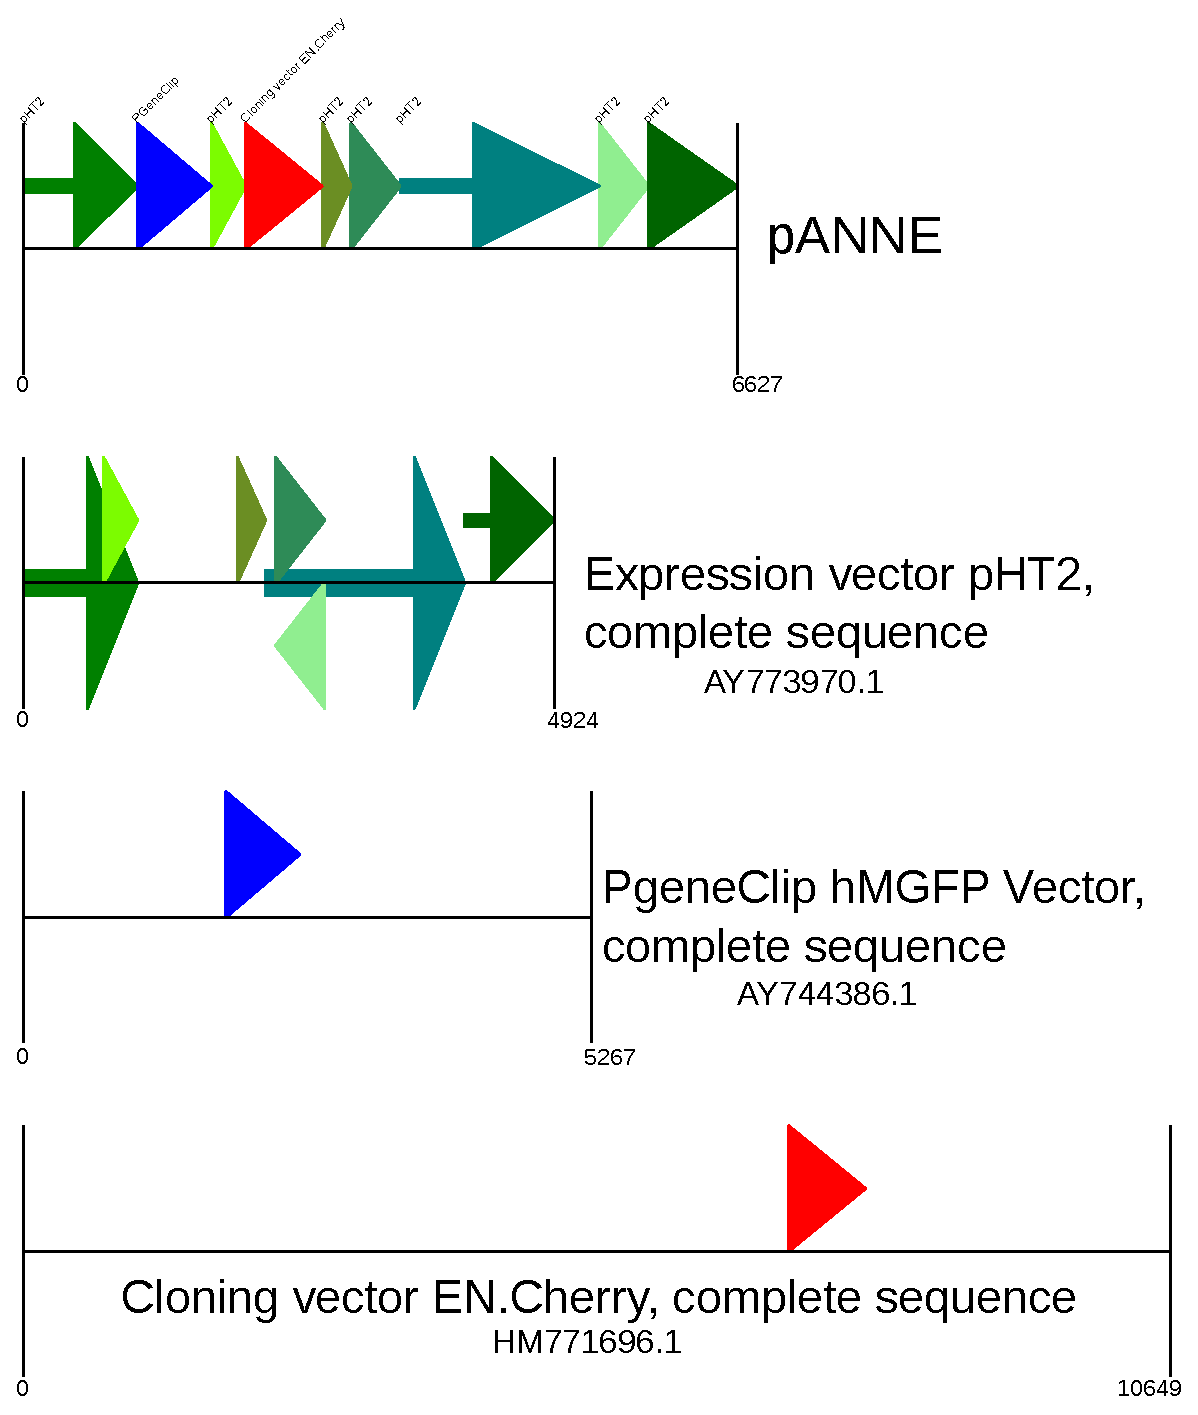
\includegraphics[width=\linewidth]{pANNE.eps}


%----------------------------------------------------------------------------------------
% SECTIONS DU DOCUMENT
%----------------------------------------------------------------------------------------
 
\section{Question 4} % Major section

{\bf Utilisez blast pour trouver des orthologues du FOXP4. Récupérer le CDS de huit orthologues.}

\subsection[Alignement multiple]{Alignez ces CDS en utilisant ClustalW, dialign et Mavid}

Afin de trouver huit orthologues du gène FOXP4, j'ai tout d'abord cherché ce gène dans la base de données des
gènes de NCBI. Une série de résultat était disponible pour ce gène, chez différentes espèces. J'ai choisi de
trouver des orthologues du gène chez l'humain. J'ai donc choisi la page du gène FOXP4 chez l'homo sapiens,
et j'ai ensuite chargé le fichier genbank de la séquence référence de ce gène.

À partir du fichier genbank, j'ai demandé à NCBI de blaster la région sur la base de données nr. J'ai tout
d'abord tenter d'utiliser blastn, toutefois après cinq minutes NCBI a arrêté la recherche car elle prenait
trop de mémoire. J'ai alors utilisé l'option megablast pour avoir des séquences hautement similaire
(graphique du résultat en annexe \ref{15}). J'ai alors analysé les résultats pour obtenir les CDS de huit 
orthologues. J'ai donc laissé de côté tous les résultats chez l'humain, et aussi tous les résultats dont
les fichiers genbank ne contenait pas d'annotation pour des CDS. Pour les séquences choisies, j'ai aussi
ignorer les courtes séquences, et je me suis concentrer sur le résultat principal.

Les huit séquences choisies proviennent des expèces suivantes: Pan troglodytes, Pan paniscus, Gorilla gorilla,
Pongo abelii, Nomascus Leucogenys, Macaca fascicularis, Macaca mulatta et Saimiri bolivensis. Pour chacune
des espèces, j'ai vérifié les annotations du fichier genbank pour m'assurer que le CDS du fichier correspondait
au gène FOXP4. J'ai ensuite téléchargé les CDS en format fasta, tel qu'offert par l'interface de NCBI.
Finalement, j'ai créé un fichier multiple fasta pour ces 8 séquences en copiant/collant dans un nouveau fichier
le contenu des 8 fichiers.

J'ai ensuite installé les trois logiciels sur mon ordinateur (information sur le système en annexe \ref{16}).

\subsection[Facilité et rapidité des programmes]{Discutez de la performance en terme de facilité d'utilisation
et de rapidité des différents programmes.}

J'ai d'abord testé clustalw. J'ai utilisé la commande suivante pour lancer l'alignement: 
\texttt{time clustalw2 foxp4\_ortho.fa $>$ clustalw.log} (log de l'alignement en annexe \ref{17}). Ensuite,
j'ai fait le même processus avec dialign. J'ai utilisé la commande suivante pour lancer l'alignement:
\texttt{time dialign -n foxp4\_ortho.fa}. Ici, le programme ne produit pas de texte pour ce qu'il fait. J'ai
utilisé l'option -n car je tentais d'aligner des séquences nucléotidiques, et non des séquences de protéine,
ce qui est le défaut de dialign.

Finalement, j'ai effectué l'alignement avec Mavid. Le processus fut beaucoup plus difficile. J'ai tout d'abord
tenté de lancé mavid avec seulement le fichier multifasta. Mavid a donné une erreur, car il s'attendait à
recevoir aussi un fichier d'arbre phylogénique en format Newick. En regardant la documentation, je me
suis rendu compte que Mavid contient un programme pour créer l'arbre. Il suffisait d'utiliser le script
Perl pour créer l'arbre et ensuite lancé Mavid. Après avoir mis à jour les chemins dans le script Perl,
j'ai tenté de nouveau de lancé Mavid. Encore une fois, l'application a donné une erreur, s'attendant à
avoir un repeat masking file, de RepeatMasker. J'ai alors téléchargé l'application, et j'ai tenté de
l'installé localement. Toutefois, RepeatMasker doit se connecter sur un moteur de recherche, et je n'ai
pas réussi à effectuer cette partie de l'installation.

J'ai donc décidé de chercher s'il est possible d'utiliser RepeatMasker en ligne. Le site RepeatMasker permet
son utilisation en ligne, j'ai donc tenté d'obtenir un fichier de masque pour mes séquences. Toutefois, j'ai
toujours obtenu le même résultat pour mes recherches: aucune séquence répété dans mon fichier fasta (voir \ref{18}).
J'ai donc tenté de créer un fichier de masquage vide pour les séquences. Toutefois, avec le peu d'information disponible,
j'ai mis beaucoup de temps à comprendre qu'un fichier de masquage sans séquences répétés est seulement un fichier
fasta identique au fichier original, avec l'extension .masked. Finalement, j'ai alors réussi à faire fonctionner
Mavid (log de l'exécution en annexe \ref{19}). Comme on peut le constater, Mavid fait appel à clustalw durant son
exécution.

La rapidité d'exécution des applications est disponible en annexe \ref{24}. Mavid semble le programme le plus rapide pour
créer l'alignement, toutefois son manque de documentation rend son utilisation très difficile. Dialign est plus lent,
il pourrait aussi donner plus d'information à l'utilisateur sur son fonctionnement. ClustalW semble être relativement
rapide, tout en étant facile à utiliser.

\subsection[Qualité des alignements]{Analysez et discutez de la qualité de l'alignement donné par chaque méthode.}

Regardons d'abord le résutlat obtenu par ClustalW. À première vue, l'alignement semble être en grande majorité de qualité,
on y remarque très peu de gap et de mismatch. On peut s'attendre à ce résultat selon l'arbre phylogénique
créé par ClustalW. En général, ClustalW donne un résultat de qualité si on utilise des séquences partageant un ancêtre commun.
Comme nous avons choisi des orthologues d'un gène, on peut donc s'attendre à un résultat de qualité. Comme on peut le voir en
\ref{20}, la distance dans l'arbre phylogénique est assez petite ici, on peut donc s'attendre à un résultat de qualité.

Les repères pour la qualité de dialign sont plus difficiles à évaluer. Le programme crée lui aussi un arbre phylogénique (\ref{21}),
qui est beaucoup plus balancé que celui de ClustalW. En regardant le fichier de sortie, on peut remarquer des scores 
d'alignement assez élevé pour la majorité du fichier, on retrouve à quelques endroits une série de gap, mais en général le résultat
semble très similaire à celui de ClustalW.

Finalement, le fichier d'alignement créé par Mavid ne contient aucune information à propos de l'alignement. Mavid produit un fichier
mfa, donc multiple fasta, où on peut remarquer des gaps assez long à certains endroits. Pour plus d'information, Mavid produit
aussi un fichier phylip plus facile à analyser. On y remarque certaines régions de gap, mais il est très difficile
de remarquer les mismatchs. L'arbre phylogénique produit (\ref{22}) ressemble à celui de Dialign, mais les distances entre les
espèces n'est pas aussi grand.

\subsection[Meilleur alignement]{Quel est votre meilleur alignement? Justifiez votre choix.}

Le choix d'un alignement dépend de ce qu'on veut en faire. Pour en faire une analyse plus poussée, il est
généralement nécessaire d'éditer l'alignement multiple, selon les connaissances des séquences qui ont été
alignées. Un choix d'alignement pourrait donc être basé sur la minimisation du travail d'édition à faire
sur le résultat.

On peut donc éliminer l'alignement de Mavid, car le format mfa qu'il produit semble nécessiter plus de
travail, ne serait-ce que pour avoir une représentation montrant clairement où sont les mismatchs.

Il est plus difficile de départager entre les alignements de ClustalW et Dialign. Selon Mower et Annaiah, 
Dialign semble excellé lorsque les séquences ont une distance évolutive très élevées. Ce n'est pas le cas
ici, donc il serait préférable de prendre l'alignement multiple produit par ClustalW. De plus, ClustalW
produit un résultat plus rapidement que Dialign. Ce n'est pas un critère très important ici, car
les séquences alignées sont assez courtes, mais pour des séquences plus longues, ce serait un
point à considérer.

\begingroup
\renewcommand{\appendix}{%
    \renewcommand{\thesubsection}{\arabic{subsection}}
}

\newpage
\appendix
\section{Annexes}
\subsection{Image du locus du gène ALS2 chez l'homo sapien du UCSC genome browser}\label{1}
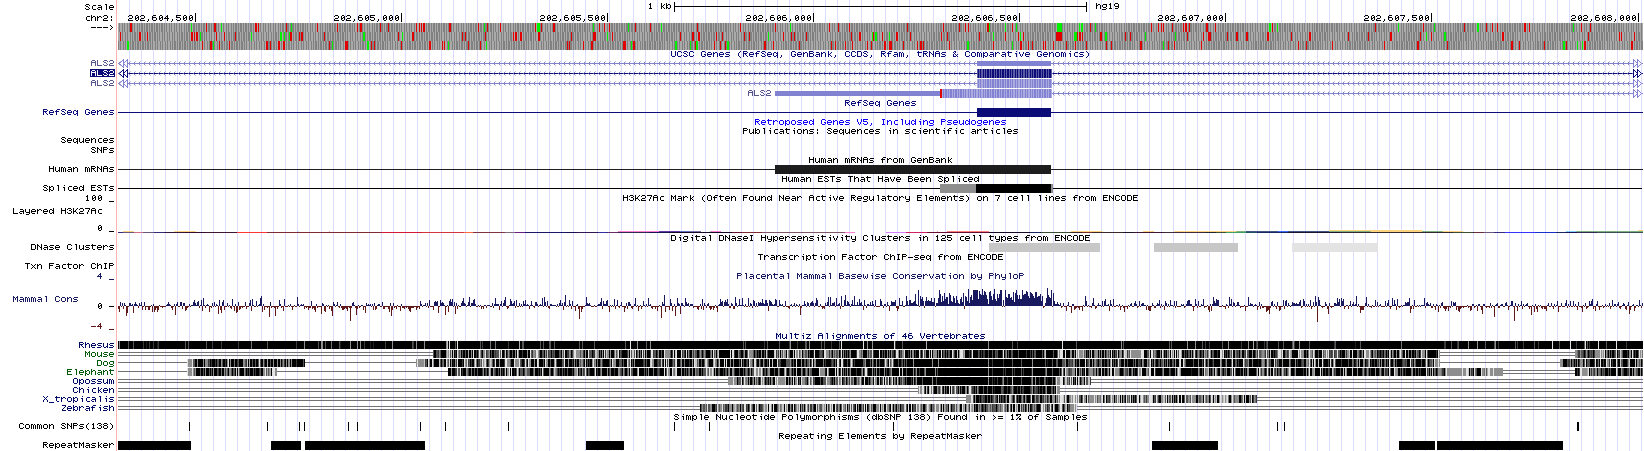
\includegraphics[width=\linewidth]{annexes/annexe1_ucsc.png}

\subsection{Image du locus du gène ALS2 chez l'homo sapien de NCBI}\label{2}
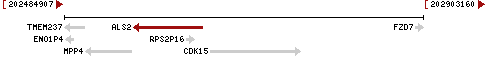
\includegraphics{annexes/annexe1_ncbi_als2.png}

\subsection{Script biopython de calcul des fréquences nucléotidiques}\label{3}
\begin{lstlisting}[frame=single,numbers=left,language=Python]
# -* coding:utf-8 *-#
from Bio import SeqIO
from Bio.SeqRecord import SeqRecord
handle = open("NC_000002_202564986-202645895.gb", "r")
seq_record = SeqIO.parse(handle, 'gb')
for seq in seq_record:
    dist_a = seq.seq.count("A")
    dist_c = seq.seq.count("C")
    dist_g = seq.seq.count("G")
    dist_t = seq.seq.count("T")
    print "A:  count: " + str(dist_a) + " % = " + \
        str(float(dist_a)/len(seq)*100)
    print "C:  count: " + str(dist_c) + " % = " + \
        str(float(dist_c)/len(seq)*100)
    print "G:  count: " + str(dist_g) + " % = " + \
        str(float(dist_g)/len(seq)*100)
    print "T:  count: " + str(dist_t) + " % = " + \
        str(float(dist_t)/len(seq)*100)
    print "total = " + str(dist_a+dist_c+dist_g+dist_t)
\end{lstlisting}

\subsection{Vue de MapViewer du locus du gène ALS2 chez l'humain, 202,555 à 202,656.}\label{4}
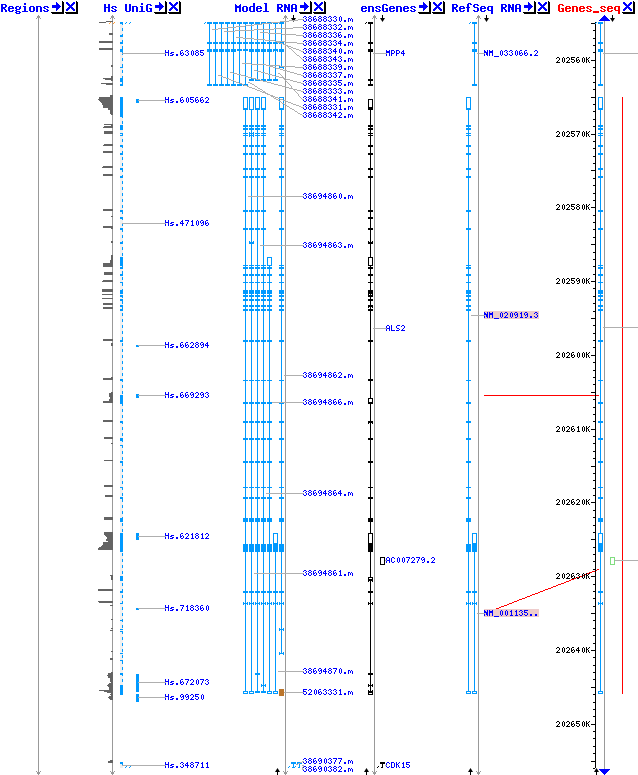
\includegraphics[width=\linewidth]{annexes/annexe1b_mapviewer_202555-202656.png}

\subsection{Vue de MapViewer du locus du gène ALS2 chez l'humain, 202M à 203M.}\label{5}
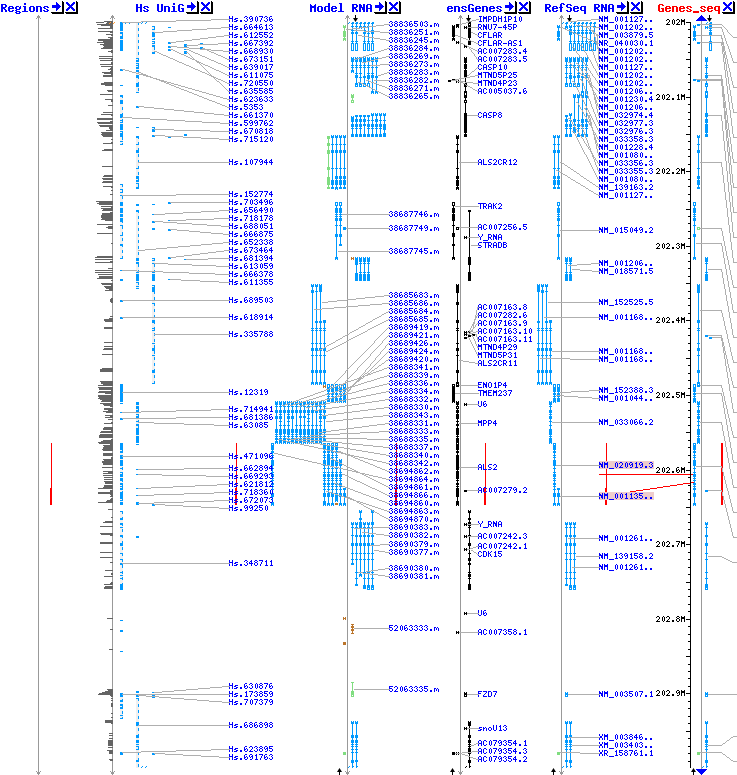
\includegraphics[width=\linewidth]{annexes/annexe1b_mapviewer_202M-203M.png}

\subsection{Vue de SequenceViewer du locus du gène ALS2.}\label{6}
%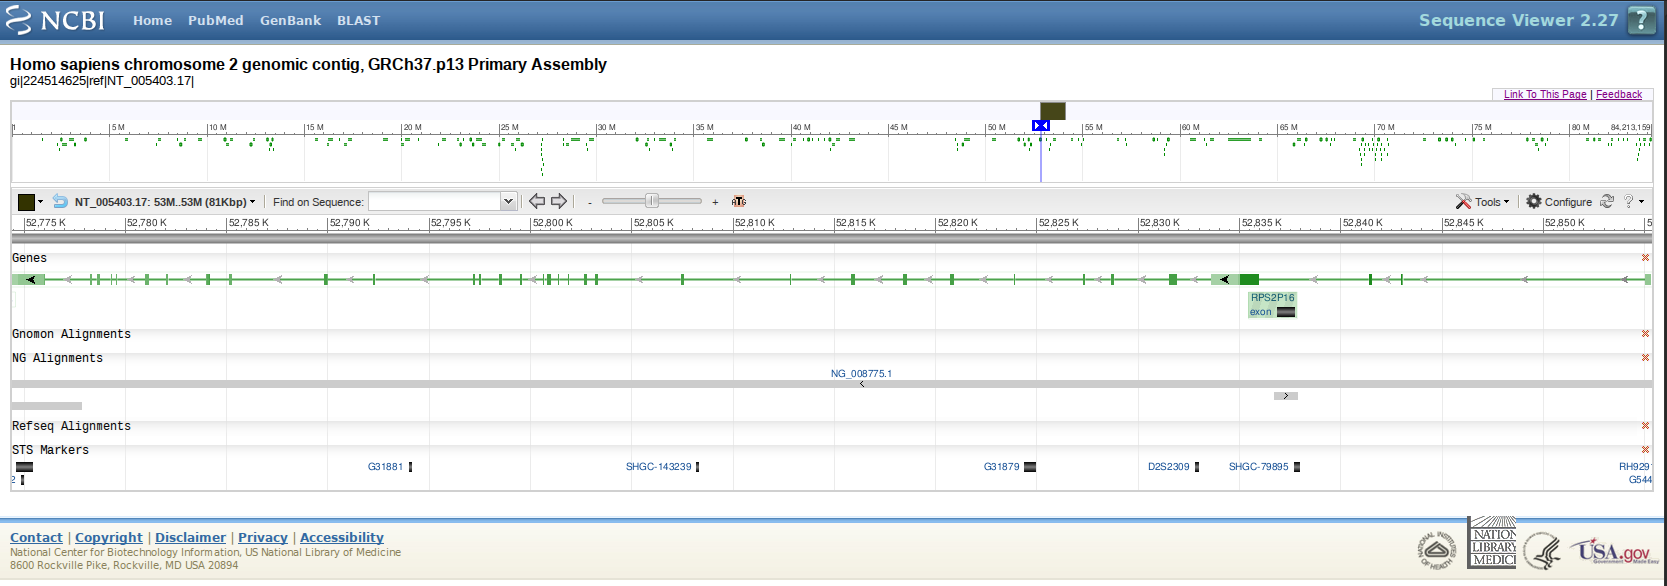
\includegraphics[width=\linewidth]{annexes/annexe1_c_sw.png}

\subsection{Script biopython Pour choisir 5 contigs au hasard à partir du résulat de CAP3, et d'effectuer
un blast sur ces contigs}\label{7}
\begin{lstlisting}[frame=single,numbers=left,language=Python]
# *- coding:utf-8 -* #
import random
from Bio.Blast import NCBIWWW

contigs = {}
contig_no = None
contig_seq = ""
contig_size = 0

with open("seq.data.cap.contigs", "r") as f:
    for line in f:
        # on regarde d'abord si c'est un contig ou non
        if line[0] == '>':
            if contig_no == None:
                contig_no = int(line[7:])
            if contig_seq != "":
                contigs.update({contig_no:contig_seq})
                contig_seq = ""
                contig_no = int(line[7:])
                contig_size+= 1
        else :
            contig_seq = contig_seq + line.replace("\n","")
    contigs.update({contig_no:contig_seq})
    contig_size +=1

# Maintenant, on a nos contigs, on en choisit 5 au hasard
random_contig = []

#Je m'assure ici de ne pas avoir de doublon
for i in range(5):
    random_c = random.randint(1, contig_size)
    while random_c in random_contig:
        random_c = random.randint(1,contig_size)
    random_contig.append(random_c)

#On blast maintenant les contigs choisis:
for i in random_contig:
    result_handle = NCBIWWW.qblast("blastn", "nr", contigs[i])

    #on enregistre le résultat
    nom_fichier = "blast_contig_" + str(i) + ".xml"
    save_file = open(nom_fichier, "w")
    save_file.write(result_handle.read())
    save_file.close()
    result_handle.close()

print "5 contigs cherchés"
\end{lstlisting}

\subsection{Information à propos de la qualité du contig 7}\label{8}
\begin{verbatim}
>Contig7
10 25 25 25 10 0 25 25 25 25 25 25 25 25 25 25 25 25 10 25 
10 25 10 25 25 25 25 25 25 25 25 25 25 25 25 25 25 25 25 25 
25 25 25 25 25 25 25 25 25 25 25 25 25 25 25 25 25 25 25 25 
25 25 25 25 25 25 25 25 25 25 25 25 25 25 25 25 25 25 25 25 
25 25 25 25 25 25 25 25 25 10 10 10 10 10 10 10 10 10 10 10 
10 25 25 25 25 25 25 25 25 25 25 25 25 25 25 25 25 10 10 10 
25 25 25 25 25 25 25 25 25 25 25 25 25 25 25 25 25 25 25 25 
25 25 25 25 25 25 25 25 25 25 25 25 25 25 25 25 25 25 25 25 
25 10 25 10 25 25 25 25 25 25 25 25 10 25 25 25 25 25 25 25 
25 25 25 25 25 25 25 25 25 25 25 25 25 25 25 25 25 25 25 25 
25 25 25 25 25 25 25 25 25 25 25 25 25 25 25 25 25 25 25 25 
25 25 25 25 25 25 25 25 25 25 25 25 25 25 25 25 25 25 25 25 
25 25 25 25 25 25 25 25 25 25 25 25 25 25 25 25 25 25 25 25 
25 25 25 25 25 25 25 25 25 25 25 25 25 25 25 25 25 25 25 25 
25 25 25 25 25 25 25 25 25 25 25 25 25 25 25 25 25 25 25 25 
25 25 25 25 25 25 25 25 25 25 25 25 25 25 25 25 25 25 25 25 
25 25 25 25 25 25 25 25 25 25 25 25 25 25 25 25 25 25 25 25 
25 25 25 25 25 25 25 25 25 25 25 25 25 25 25 25 25 25 25 25 
10 25 25 25 25 25 25 25 25 25 25 25 25 25 25 25 25 25 25 25 
25 25 25 25 25 25 25 25 25 25 25 25 25 25 25 25 25 25 25 25 
25 25 25 25 25 25 25 25 25 25 25 25 25 25 25 25 25 25 25 25 
25 25 25 25 25 25 25 25 25 25 25 25 25 25 25 25 25 25 25 25 
25 25 25 25 25 25 25 25 25 25 25 25 25 25 25 25 25 25 25 25 
25 25 25 25 25 25 25 25 25 25 25 25 25 25 25 25 25 25 25 25 
25 25 25 25 25 25 25 25 25 25 25 25 25 25 25 25 25 25 25 25 
25 25 25 25 25 25 25 25 25 25 25 25 25 25 25 25 25 25 25 25 
25 25 25 25 10 25 25 25 25 25 25 25 25 25 25 25 25 25 25 25 
25 25 25 25 25 25 25 25 25 25 25 25 25 25 25 25 25 25 25 25 
25 25 25 25 25 25 25 25 25 25 25 25 25 25 25 25 25 25 25 25 
25 25 25 25 25 25 25 25 25 25 25 25 25 25 25 25 25 25 25 25 
25 25 25 25 25 25 25 25 25 25 25 25 25 25 25 25 25 25 25 25 
25 25 25 25 25 25 25 25 25 25 25 25 25 25 25 25 10 25 25 25 
25 25 25 25 25 25 25 25 25 25 25 25 10 10 25 25 25 25 25 25 
25 25 25 25 25 25 25 25 25 25 25 25 0 25 25 25 0 25 25 10 
10 10 25 10 25 25 25 25 25 25 25 25 10 25 25 25 25 25 25 25 
25 25 25 10 25 25 10 25 25 25 25 10 25 10 25 25 10 0 25 25 
25 25 25 25 25 25 25 25 25 25 25 25 25 25 25 25 25 25 25 25 
25 25 25 25 25 25 0 25 25 25 25 10 0 10 10 25 25 25 10 25 
0 25 25 25 25 25 25 25 25 25 25 10 25 25 25 25 25 25 25 10 
0 25 25 25 25 10 25 25 25 25 25 25 25 25 10 25 25 10 25 25 
25 25 25 25 25 25 25 25 25 25 25 25 25 25 10 10 25 25 0 25 
25 25 10 25 25 25 10 25 25 25 25 25 25 25 25 10 25 25 25 10 
10 25 10 25 25 25 25 25 25 25 25 10 25 10 25 25 25 25 25 25 
0 5 15 15 15 15 15 15 15 15 15 15 15 15 15 15 15 15 10 10 
10 10 10 10 10 10 10 10 

\end{verbatim}
\subsection{Information à propos de la qualité du contig 132}\label{9}
\begin{verbatim}
>Contig132
10 10 10 10 10 10 10 10 10 10 10 10 15 15 15 15 15 15 15 15 
15 15 15 15 15 15 15 15 15 15 15 15 15 15 15 15 15 15 15 15 
15 15 15 15 15 15 15 15 15 15 15 15 15 15 15 15 15 15 15 15 
15 15 15 15 15 15 15 15 15 15 15 0 0 0 0 0 15 15 15 15 
15 15 15 15 15 15 15 15 20 20 20 20 20 20 20 20 20 20 20 20 
20 20 20 20 20 20 20 20 20 20 20 20 20 20 20 20 20 20 20 20 
20 20 20 20 20 20 20 20 20 20 20 20 20 20 20 20 20 20 20 20 
20 20 20 20 20 20 20 20 20 20 20 20 20 20 20 20 20 20 20 20 
20 20 20 20 20 20 20 20 20 20 20 20 20 20 20 20 20 20 20 20 
20 20 20 20 20 20 20 20 20 20 20 20 20 20 20 20 20 20 20 20 
20 20 20 20 20 20 20 20 20 20 20 20 20 20 20 20 20 20 20 20 
20 20 20 20 20 20 20 20 20 20 20 20 20 20 20 20 20 20 20 20 
20 20 20 20 20 20 20 20 20 20 20 20 20 20 20 20 20 20 20 20 
20 20 20 20 20 20 20 20 20 20 20 20 20 20 20 20 20 20 20 20 
20 20 20 20 20 20 20 20 20 20 20 20 20 20 20 20 20 20 20 20 
20 20 20 20 20 20 20 20 20 20 20 20 20 20 20 20 20 20 20 20 
20 20 20 20 20 20 20 20 20 20 20 20 20 20 20 20 20 20 20 20 
20 20 20 20 20 20 20 20 20 20 20 20 20 20 20 20 20 20 20 20 
20 20 20 20 20 20 20 20 20 20 20 20 20 20 20 5 20 20 20 20 
20 20 20 20 20 20 20 20 20 20 20 20 20 20 20 20 20 20 20 20 
20 20 20 20 20 20 20 20 20 20 20 20 20 20 20 20 20 20 20 20 
20 20 20 20 20 20 20 20 20 20 20 20 20 20 20 20 20 20 20 20 
20 20 20 20 20 20 20 20 20 20 20 20 20 20 20 20 20 20 20 20 
20 20 20 20 20 20 20 20 20 20 20 20 20 20 20 20 20 20 20 20 
20 20 20 20 20 20 20 20 20 20 20 20 20 20 20 20 20 20 20 20 
20 20 20 20 20 20 20 20 20 20 20 20 20 20 20 20 20 20 20 20 
20 20 20 20 20 20 20 20 20 20 20 20 20 20 20 20 20 20 20 20 
20 20 20 20 20 20 20 20 20 20 20 20 20 20 20 20 20 20 20 20 
20 20 20 20 20 20 20 20 20 20 20 20 20 20 20 20 20 20 20 20 
20 20 20 20 20 20 20 20 20 20 20 20 20 20 20 20 20 20 20 20 
20 20 20 20 20 20 20 20 20 20 20 20 20 20 20 20 20 20 20 20 
20 20 20 20 20 20 20 20 20 20 20 20 20 20 20 20 20 20 20 20 
20 20 20 20 20 20 20 20 20 20 20 20 20 20 20 20 20 20 20 20 
20 20 20 20 20 20 20 20 20 20 20 20 20 20 20 20 20 20 20 20 
20 20 20 20 20 20 20 20 20 20 20 20 20 20 20 20 20 20 20 20 
20 20 20 20 20 20 20 20 20 20 20 20 20 20 20 20 20 20 20 20 
20 20 20 20 20 20 20 20 20 20 20 20 20 20 20 20 20 20 20 20 
20 20 20 20 20 20 20 0 20 20 5 20 20 20 20 20 20 20 20 20 
20 5 20 20 20 20 15 15 15 15 0 15 15 15 15 15 15 15 15 15 
15 15 15 15 15 15 15 15 15 15 15 15 15 15 15 15 15 15 15 15 
0 15 15 15 15 15 15 15 0 0 15 15 15 0 15 15 15 0 15 15 
15 15 15 15 15 15 15 0 0 0 0 15 15 15 15 15 15 15 15 15 
15 15 0 15 15 15 15 15 15 15 15 0 15 15 0 15 15 15 15 0 
15 15 15 0 15 15 15 15 15 15 15 15 0 15 15 15 15 0 15 15 
15 0 15 0 15 15 15 15 0 15 15 15 15 15 15 15 15 15 15 15 
15 0 15 15 15 15 15 15 15 15 15 15 15 15 15 15 0 0 15 15 
15 15 15 15 15 15 15 15 15 15 15 15 15 15 0 15 0 15 15 15 
0 15 15 15 15 15 15 10 10 10 10 10 10 10 10 10 10 10 10 10 
10 10 10 10 10 10 10 10 10 10 10 10 10 10 10 10 10 10 10 10 
10 10 10 10 10 10 10 10 10 10 10 10 10 10 10 10 10 10 10 10 
10 10 10 10 10 10 10 10 10 10 10 10 10 10 10 10 10 10 10 10 
10 10 10 10 10 10 10 10 10 10 10 10 10 10 10 10 10 10 10 10 
10 10 10 10 10 10 10 10 10 10 10 10 10 10 10 10 10 10 10 10 
10 10 10 10 10 10 10 10 10 10 10 10 10 10 10 10 10 10 10 10 
10 10 10 10 10 10 10 10 10 10 10 10 10 10 10 10 10 10 10 10 
10 10 10 10 10 10 10 10 10 10 10 10 10 10 10 10 10 10 10 10 
10 10 10 10 10 10 10 10 10 10 10 10 10 10 10 10 10 10 10 10 
10 10 10 10 10 10 10 10 10 10 10 10 10 10 10 10 10 10 10 10 
10 10 10 10 10 10 10 10 10 10 10 10 10 10 10 10 10 10 10 10 
10 10 10 10 10 10 10 10 10 10 10 10 10 10 10 10 10 10 10 10 
10 10 10 10 10 10 10 10 10 10 10 10 10 10 10 10 10 
\end{verbatim}
\subsection{Information à propos de la qualité du contig 195}\label{10}
\begin{verbatim}
>Contig195
15 0 15 15 15 15 0 15 15 15 15 15 15 15 15 15 15 0 15 15 
15 15 15 15 15 15 15 15 15 15 15 15 15 15 15 15 15 15 15 15 
15 15 15 15 15 15 15 15 15 15 15 15 15 15 15 15 15 15 15 15 
15 15 15 15 15 15 15 15 15 15 15 15 15 15 15 15 15 15 15 15 
15 15 15 15 15 15 15 15 15 15 0 0 0 0 0 0 0 0 0 0 
0 0 0 0 0 0 15 15 15 15 15 15 15 15 15 15 15 15 15 15 
15 15 15 15 15 15 15 15 15 15 15 15 15 15 15 15 15 15 15 15 
15 15 15 15 15 15 15 15 15 15 15 15 15 15 15 15 15 15 15 15 
15 15 15 15 15 15 15 15 15 15 15 15 15 15 15 15 15 15 15 15 
15 15 15 15 15 15 15 15 15 15 15 15 15 15 15 15 15 15 15 15 
15 15 15 15 15 15 15 15 15 15 15 15 15 15 15 15 15 15 15 15 
15 15 15 15 15 15 15 15 15 15 15 15 15 15 15 15 15 15 15 15 
15 15 15 15 15 15 15 15 15 15 15 15 15 15 15 15 15 15 15 15 
15 15 15 15 15 15 15 15 15 15 0 15 15 15 15 15 15 15 15 15 
15 15 15 15 15 15 15 15 15 15 15 15 15 15 15 15 15 15 15 15 
15 15 15 15 15 15 15 15 15 15 15 15 15 15 15 15 15 15 15 15 
15 15 15 15 15 15 15 15 15 15 15 15 15 15 15 15 15 15 15 15 
15 15 15 15 15 15 15 15 15 15 15 15 15 15 15 15 15 15 15 15 
15 15 15 15 15 15 15 15 15 15 15 15 15 15 15 15 15 15 15 15 
15 15 15 15 15 15 15 15 15 15 15 15 15 15 15 15 15 15 15 15 
15 15 15 15 15 15 15 15 15 15 15 15 15 15 15 15 15 15 15 15 
15 15 15 15 15 15 15 15 15 15 15 15 15 15 15 15 0 15 15 15 
15 15 15 15 15 15 15 15 15 15 15 15 15 15 15 15 15 15 15 15 
15 15 15 15 15 15 0 15 15 15 15 15 15 15 15 15 15 15 15 15 
15 15 15 15 15 15 15 15 15 15 15 15 15 15 15 15 15 15 15 15 
15 15 15 15 15 15 15 15 15 15 15 15 15 15 15 15 15 15 15 15 
15 15 15 15 15 15 15 15 15 15 15 15 15 15 15 15 15 15 15 15 
15 15 15 15 15 15 15 15 15 15 15 15 15 15 15 15 15 15 15 15 
15 15 15 15 15 15 15 15 15 15 15 15 15 15 15 15 15 15 15 0 
15 15 15 15 15 15 15 15 15 15 15 15 15 15 15 15 15 15 15 15 
15 15 0 15 15 15 15 15 15 15 15 15 15 15 15 15 15 0 15 15 
15 15 15 15 15 15 15 15 15 15 15 15 15 15 15 15 15 15 15 15 
15 15 15 15 15 15 15 15 15 15 15 15 15 15 15 15 15 15 15 15 
0 15 15 15 15 15 15 15 15 15 0 15 15 15 15 15 15 15 15 15 
15 15 15 15 15 15 15 15 15 15 15 15 15 15 15 15 15 15 15 15 
15 15 15 15 15 15 15 15 15 15 15 15 15 15 15 15 0 15 15 15 
15 15 15 15 15 15 15 15 15 15 15 15 15 15 15 15 15 15 15 15 
15 15 15 15 15 0 15 15 0 15 15 15 15 15 15 15 15 15 15 15 
15 15 15 15 15 15 15 15 15 15 15 15 15 15 15 15 15 15 15 15 
15 15 15 25 25 25 25 25 25 25 25 25 20 20 20 20 20 20 20 20 
20 20 20 0 0 20 20 20 20 20 0 20 20 20 20 20 20 20 20 20 
20 20 20 20 20 20 20 20 20 20 20 20 20 20 20 20 20 20 20 20 
20 20 20 20 20 20 20 20 20 20 20 20 20 20 20 20 20 20 20 20 
20 10 10 10 10 10 10 10 10 10 10 10 10 10 10 10 10 10 10 10 
10 10 10 10 10 10 10 10 10 10 10 10 10 10 10 10 10 10 10 10 
10 10 10 10 10 10 10 10 10 10 10 10 10 10 10 10 10 10 10 10 
10 10 10 10 10 10 10 10 10 10 10 10 10 10 10 10 10 10 10 10 
10 10 10 10 10 10 10 10 10 10 10 10 10 10 10 10 10 10 10 10 
10 10 10 10 10 10 10 10 10 10 10 10 10 10 10 10 10 10 10 10 
10 10 10 10 10 10 10 10 10 10 10 10 10 10 10 10 10 10 10 10 
10 10 10 10 10 10 10 10 10 10 10 10 10 10 10 10 10 10 10 10 
10 10 10 10 10 10 10 10 10 10 10 10 10 10 10 10 10 10 10 10 
10 10 10 10 10 10 10 10 10 10 10 10 10 10 10 10 10 10 10 10 
10 10 10 10 10 10 10 10 10 10 10 10 10 10 10 10 10 10 10 10 
10 10 10 10 10 10 10 10 10 10 10 10 10 10 10 10 10 10 10 10 
10 10 10 10 10 10 10 10 10 10 10 10 10 10 10 10 10 10 10 10 
10 10 10 10 10 10 10 10 10 10 10 10 10 10 10 10 10 10 10 10 
10 10 10 10 10 10 10 10 10 10 10 10 10 10 10 10 10 10 10 10 
10 10 10 10 10 10 10 10 10 10 10 10 10 10 10 10 10 10 10 10 
10 10 10 10 10 10 10 10 10 10 10 10 10 10 10 10 10 10 10 10 
10 10 10 10 10 10 10 10 10 10 10 10 10 10 10 10 10 10 10 10 
10 10 10 10 10 10 10 10 10 10 10 10 10 10 10 10 10 10 10 10 
10 10 10 10 10 10 10 10 10 10 10 10 10 10 10 10 10 10 10 10 
10 10 10 10 10 10 10 10 10 10 10 10 10 10 10 10 10 10 10 10 
10 10 10 10 10 10 10 10 10 10 10 10 10 10 10 10 10 10 10 10 
10 10 10 10 10 10 10 10 10 10 10 10 10 10 10 10 10 10 10 10 
10 10 10 10 10 10 10 10 10 10 10 10 10 10 10 10 10 10 10 10 
10 10 10 10 10 10 10 10 10 10 10 10 10 10 10 10 10 10 10 10 
10 10 10 10 10 10 10 10 10 10 10 10 10 10 10 10 10 10 10 10 
10 10 10 10 10 10 10 10 10 10 10 10 10 10 10 10 10 10 10 10 
10 10 10 10 10 10 10 10 10 10 10 10 10 10 10 10 10 10 10 10 
10 10 10 10 10 10 10 10 10 10 10 10 10 10 10 10 10 10 10 10 
10 10 10 10 10 10 10 10 10 10 10 10 10 10 10 10 10 10 10 10 
10 10 10 10 10 10 10 10 10 10 10 10 10 10 10 10 10 10 10 10 
10 10 10 10 10 10 10 10 10 10 10 10 10 10 10 10 10 10 10 10 
10 10 10 10 10 10 10 10 10 10 10 10 10 10 10 10 10 10 10 10 
10 10 10 10 10 10 10 
\end{verbatim}

\subsection{Information à propos de la qualité du contig 209}\label{11}
\begin{verbatim}
>Contig209
10 10 25 25 10 25 10 25 25 25 25 25 25 25 25 25 25 10 25 0 
25 25 25 25 25 25 25 25 25 25 25 25 25 25 25 25 25 25 25 25 
25 25 25 25 25 25 25 25 25 25 25 25 25 25 25 25 25 25 25 25 
25 25 25 25 25 25 25 25 25 25 25 25 25 25 25 25 25 25 25 25 
25 25 25 25 25 25 25 25 10 10 10 10 10 10 25 25 25 25 25 25 
25 25 25 25 25 25 25 25 25 25 25 25 25 25 25 25 25 25 25 25 
25 25 25 25 25 25 25 25 25 25 25 25 25 25 25 25 25 25 25 25 
25 25 25 25 25 25 25 25 25 25 25 25 25 25 25 25 25 25 25 25 
25 25 25 25 25 25 25 25 25 25 25 25 25 25 25 25 25 25 25 25 
25 25 25 25 25 25 25 25 25 10 25 25 25 25 25 25 25 10 25 25 
25 25 25 25 25 25 25 25 25 25 25 25 25 25 25 25 25 25 25 25 
25 25 25 25 25 25 25 25 25 25 25 25 25 25 25 25 25 25 25 25 
25 25 25 25 25 25 25 25 25 25 25 25 25 25 25 25 25 25 25 25 
25 25 25 25 25 25 25 25 25 25 25 25 25 25 25 25 25 25 25 25 
25 25 25 25 25 25 25 25 25 25 25 25 25 25 25 25 25 25 25 25 
25 25 25 25 25 25 25 25 25 25 25 25 25 25 25 25 25 25 25 25 
25 25 25 25 25 25 25 25 25 25 25 25 25 25 25 25 25 25 25 25 
25 25 25 25 25 25 25 25 25 25 25 25 25 25 25 25 25 25 25 25 
25 25 25 25 25 25 25 25 25 25 25 25 25 25 25 25 25 25 25 25 
25 25 25 25 25 25 25 25 25 25 25 25 25 25 25 25 25 25 25 25 
25 25 25 25 25 25 25 25 25 25 25 25 25 25 25 25 25 25 25 25 
25 25 25 25 25 25 25 25 25 25 25 25 25 25 25 25 25 25 25 25 
25 25 25 25 25 25 25 25 25 25 25 25 25 25 25 25 25 25 25 25 
25 25 25 25 25 25 25 25 25 25 25 25 25 25 25 25 25 25 25 25 
25 25 25 25 25 25 25 25 25 25 25 25 25 25 25 25 25 25 25 25 
25 25 25 25 25 25 25 25 25 25 25 25 25 25 25 25 25 25 25 25 
25 25 25 25 25 25 25 25 25 25 25 25 25 25 25 25 25 25 25 25 
25 25 25 25 25 25 25 25 25 25 25 25 25 25 25 25 25 25 25 25 
25 25 25 25 25 25 25 25 25 25 25 25 25 25 25 25 25 10 25 25 
25 10 25 25 25 25 25 25 25 25 25 25 25 25 25 10 25 25 25 25 
25 25 25 25 25 25 25 25 25 25 10 25 25 25 25 25 25 25 25 25 
25 25 25 25 25 25 25 10 25 25 25 25 25 25 25 25 25 25 25 25 
25 25 25 25 10 25 25 25 25 25 25 25 25 25 25 25 25 25 25 25 
25 25 25 25 25 25 10 25 25 25 25 25 10 25 25 25 25 10 25 25 
25 25 25 25 25 10 25 25 25 25 25 25 25 10 25 25 25 25 10 10 
25 25 10 10 10 25 25 25 25 0 0 25 10 10 10 25 25 25 10 25 
25 25 25 25 25 25 0 10 25 25 25 25 25 25 25 10 25 25 25 25 
25 25 25 25 25 25 25 25 25 25 25 25 10 25 25 20 20 20 20 20 
20 20 20 20 20 20 20 5 20 5 20 20 20 5 20 15 15 15 15 15 
15 15 15 15 15 15 15 15 15 15 15 15 15 15 10 10 10 10 10 10 
10 10 10 10 10 10 10 10 10 10 10 10 10 10 10 10 10 10 10 10 
10 10 10 10 10 10 10 10 10 10 10 10 10 10 10 10 10 10 10 10 
10 10 10 10 10 10 10 10 10 10 
\end{verbatim}

\subsection{Information à propos de la qualité du contig 214}\label{12}
\begin{verbatim}
>Contig214
15 15 15 15 15 15 15 15 15 15 15 15 15 15 15 15 5 5 20 20 
5 10 0 0 10 0 10 25 10 25 0 25 10 25 25 0 0 0 25 0 
25 0 0 10 0 0 10 0 25 0 0 0 0 0 0 25 25 25 25 25 
25 25 25 25 25 25 25 25 25 25 25 25 25 25 25 25 25 25 25 25 
25 25 25 25 25 25 25 25 10 0 25 10 25 10 25 25 25 25 25 25 
25 25 25 25 10 25 25 25 25 25 25 25 25 25 10 25 25 25 25 25 
25 25 25 25 25 25 25 25 25 25 25 25 25 10 25 25 25 25 25 25 
25 25 25 25 25 25 25 25 25 25 25 25 25 25 25 25 25 25 25 25 
25 25 25 25 25 25 25 25 25 25 25 25 25 25 25 25 25 25 25 25 
25 25 25 25 25 25 25 25 25 25 25 25 25 25 25 25 25 25 25 25 
25 25 25 25 25 25 25 25 25 25 25 25 25 25 25 25 25 25 25 25 
25 25 25 25 25 25 25 25 25 25 25 25 25 25 25 25 25 25 25 25 
25 25 25 25 25 25 25 25 25 25 25 25 25 25 25 25 25 25 25 25 
25 25 25 25 25 25 25 10 25 25 25 25 25 25 25 25 25 25 25 25 
25 25 25 25 25 25 25 25 25 25 25 25 25 25 25 25 25 25 25 25 
25 25 25 25 25 25 25 25 25 25 25 25 25 25 25 25 25 25 25 25 
25 25 25 25 25 25 25 25 25 25 25 25 25 25 25 25 25 25 25 25 
25 25 25 25 25 25 25 25 25 25 25 25 25 25 25 25 25 25 25 25 
25 25 25 25 25 25 25 25 25 25 25 25 25 25 25 25 25 25 25 25 
25 25 25 25 25 25 25 25 25 25 25 25 25 25 25 25 25 25 25 25 
25 25 25 25 25 25 25 25 25 25 25 25 25 25 25 25 25 25 25 25 
25 25 25 25 25 25 25 25 25 25 25 25 25 25 25 25 25 25 25 25 
25 25 25 25 25 25 25 25 25 25 25 25 25 25 25 10 25 25 25 25 
25 25 25 25 25 25 25 25 25 25 25 25 25 25 25 25 25 25 25 25 
25 25 25 25 25 25 25 25 25 25 25 25 25 25 25 25 10 25 25 25 
25 25 25 25 25 25 25 25 25 25 25 25 25 25 25 25 25 25 25 25 
25 25 25 10 25 25 25 35 35 20 35 35 35 35 35 35 35 35 15 35 
35 35 15 35 35 35 35 35 15 0 20 15 35 35 35 35 15 35 35 35 
35 35 35 35 35 35 35 20 15 20 35 35 35 35 35 35 35 15 35 35 
35 35 35 35 35 35 20 35 35 35 35 15 35 20 35 35 35 35 0 35 
35 30 30 30 30 30 30 30 30 30 30 30 30 30 30 30 30 30 30 30 
30 30 30 30 30 30 30 30 30 30 30 10 30 30 30 30 30 10 10 30 
30 30 30 30 30 30 30 30 30 30 30 30 30 30 30 30 30 10 30 30 
30 30 30 30 30 30 30 30 30 30 30 30 30 30 30 30 30 30 30 30 
30 30 30 30 30 30 30 30 30 30 30 30 30 30 30 30 30 30 30 30 
30 30 30 30 10 30 10 30 30 30 30 30 30 30 30 30 30 30 30 30 
30 30 30 30 30 30 30 30 30 30 30 30 30 30 30 30 30 15 30 30 
30 30 30 10 30 30 30 30 30 30 30 30 30 30 30 30 30 30 30 30 
30 30 30 25 25 25 25 25 25 0 20 20 20 20 20 20 20 0 20 20 
20 20 20 20 20 20 20 20 20 20 20 20 20 20 20 20 20 20 20 20 
20 20 20 20 20 20 20 20 20 20 20 20 20 20 20 20 20 20 20 20 
20 20 20 20 20 20 20 20 20 20 20 20 20 20 20 20 20 20 20 20 
20 20 20 20 20 20 20 20 20 20 20 20 20 20 20 20 20 20 20 20 
20 20 20 20 20 20 20 20 20 20 20 20 20 20 20 20 20 20 20 20 
20 20 20 20 20 20 20 20 20 20 20 20 20 20 20 20 20 20 20 20 
20 0 20 20 20 20 20 20 20 20 20 20 20 20 20 20 20 20 20 20 
20 20 20 20 20 20 20 20 20 20 20 20 20 20 20 20 20 20 20 20 
0 20 20 20 0 20 20 20 20 0 20 20 20 20 0 20 20 20 20 20 
0 20 20 20 20 20 20 20 20 20 0 0 20 20 20 20 0 20 20 20 
20 20 20 20 20 0 20 20 0 20 20 20 20 20 20 20 20 20 0 20 
20 20 0 20 20 20 20 20 20 20 20 20 20 20 20 20 20 0 20 20 
20 20 20 20 20 20 20 20 10 10 10 10 10 10 10 10 10 10 10 10 
10 10 10 10 10 10 10 10 10 10 10 10 10 10 10 10 10 10 10 10 
10 10 10 10 10 10 10 10 10 10 10 10 10 10 10 10 10 10 10 10 
10 10 10 10 10 10 10 10 10 10 10 10 10 10 10 10 10 10 10 10 
10 10 10 10 10 10 10 10 10 10 10 10 10 10 10 10 10 10 10 10 
10 10 10 10 10 10 10 10 10 10 10 10 10 10 10 10 10 10 10 10 
10 10 10 10 10 10 10 10 10 10 10 10 10 10 10 10 10 10 10 10 
10 10 10 10 10 10 10 10 10 10 10 10 10 10 10 10 10 10 10 10 
10 10 10 10 10 10 10 10 10 10 10 10 10 10 10 10 10 10 10 10 
10 10 10 10 10 10 
\end{verbatim}

\subsection{Résultat graphique bu blast des 5 contigs.}\label{13}

Contig 7\\
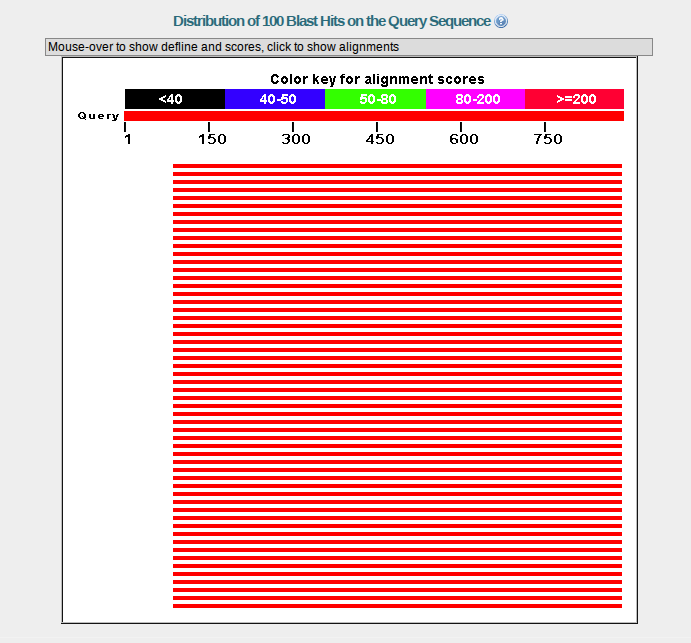
\includegraphics[width=\linewidth]{annexes/question_2/blast_contig_7_result.png}

Contig 132\\
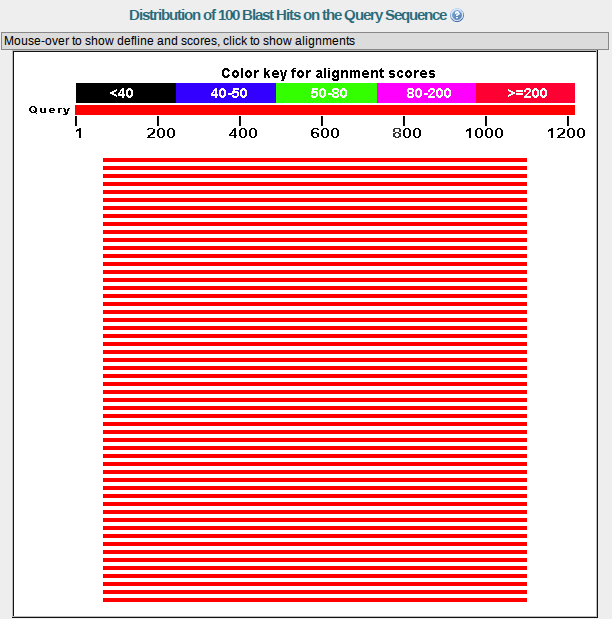
\includegraphics[width=\linewidth]{annexes/question_2/blast_contig_132_result.png}

Contig 195\\
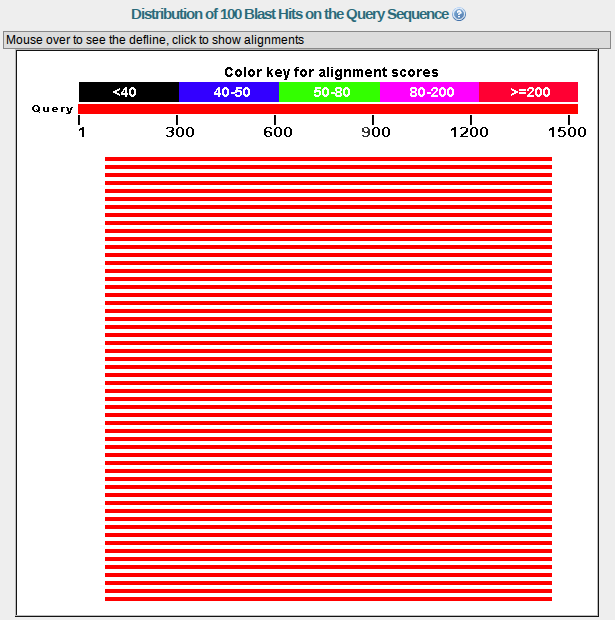
\includegraphics[width=\linewidth]{annexes/question_2/blast_contig_195_result.png}

Contig 209\\
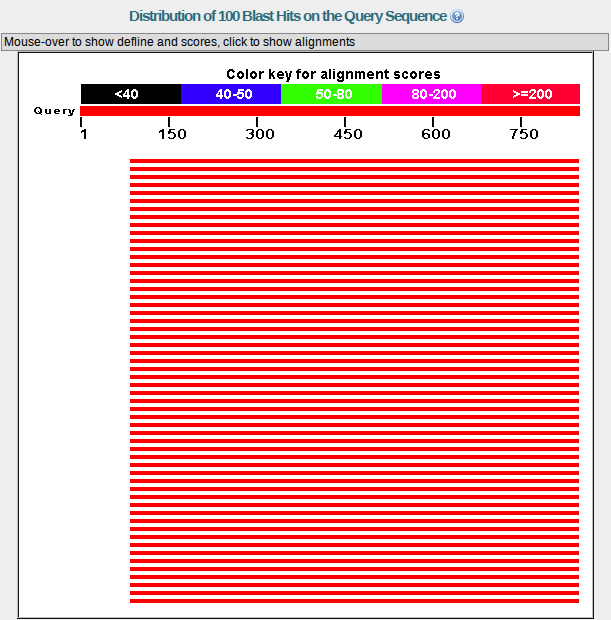
\includegraphics[width=\linewidth]{annexes/question_2/blast_contig_209_result.png}

Contig 214\\
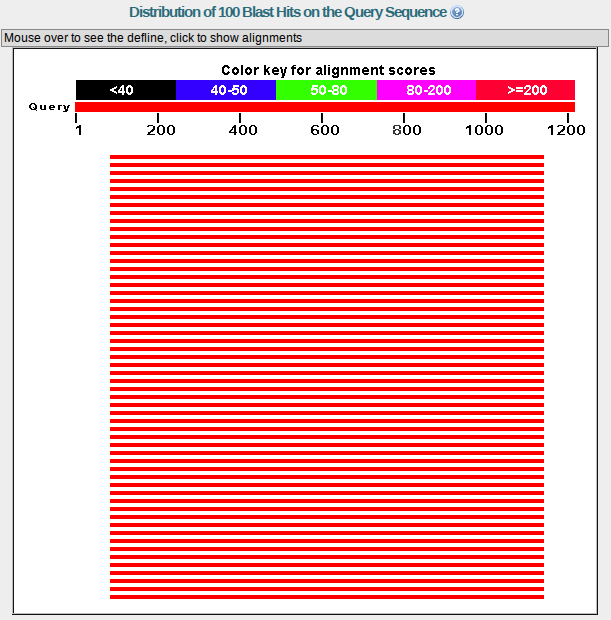
\includegraphics[width=\linewidth]{annexes/question_2/blast_contig_214_result.png}

\subsection{Script Biopython pour obtenir les fichiers d'accession des 10 premiers résultats du blast
pour un contig donné.}\label{14}
\begin{lstlisting}[frame=single,numbers=left,language=Python]
# *- coding:utf-8 -* #

#Parser pour un fichier XML de resultat blast
#Specifique a la question 2 du devoir 1. Je sais
#ici que chaque hit a seulement un hsp, donc en 
#specifiant le # d'accession et le sbjct_start et end,
#j'obtiens ce que je cherche

import sys
import os
from Bio.Blast import NCBIXML
from Bio import SeqIO
from Bio.SeqRecord import SeqRecord
from Bio import Entrez

#On choisit une E-VALUE
E_VALUE_THRESH = 0.04
Entrez.email = "glahaie@gmail.com"
path = "annexes/question_2/"

path_fichier = path + "blast_contig_"+sys.argv[1] + ".xml"

with open(path_fichier) as fichier:
    blast_record = NCBIXML.read(fichier)
    i = 0
    path_result = path + "contig_"+sys.argv[1]+"/"
    if not os.path.exists(path_result):
        os.makedirs(path_result)
    for alignment in blast_record.alignments:
        for hsp in alignment.hsps:
            if hsp.expect < E_VALUE_THRESH:
#On obtient alors le fichier genbank
                handle = Entrez.efetch(db="nucleotide", rettype="gb", 
		  retmode="text", id=alignment.accession, 
		  seq_start=hsp.sbjct_start, seq_stop=hsp.sbjct_end)
                seq_record= SeqIO.read(handle, "gb")
                handle.close()
                nom_fichier = path_result + alignment.accession + ".gb"
                SeqIO.write(seq_record, nom_fichier, "gb")

        i += 1
        if i > 10:
            break
\end{lstlisting}

\subsection{Résultat graphique bu blast du gène FOXP4 de l'Homo sapiens.}\label{15}
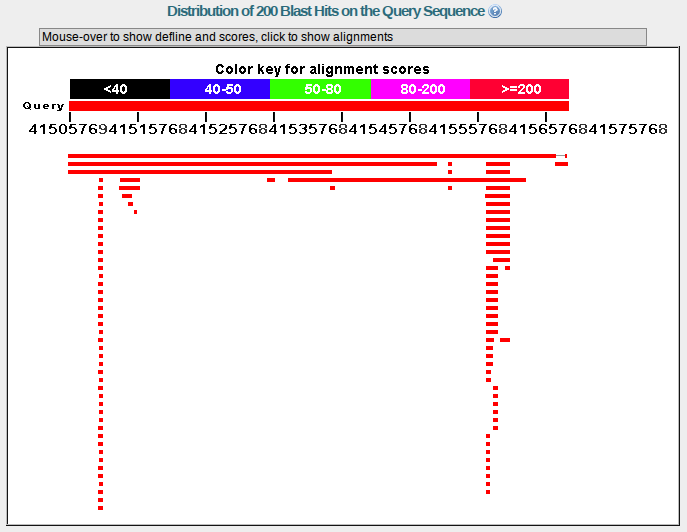
\includegraphics[width=\linewidth]{annexes/question4/FOXP4_megablast_result.png}

\subsection{Information du système qui a fait les alignements multiples.}\label{16}

Système d'exploitation et processeurs\\
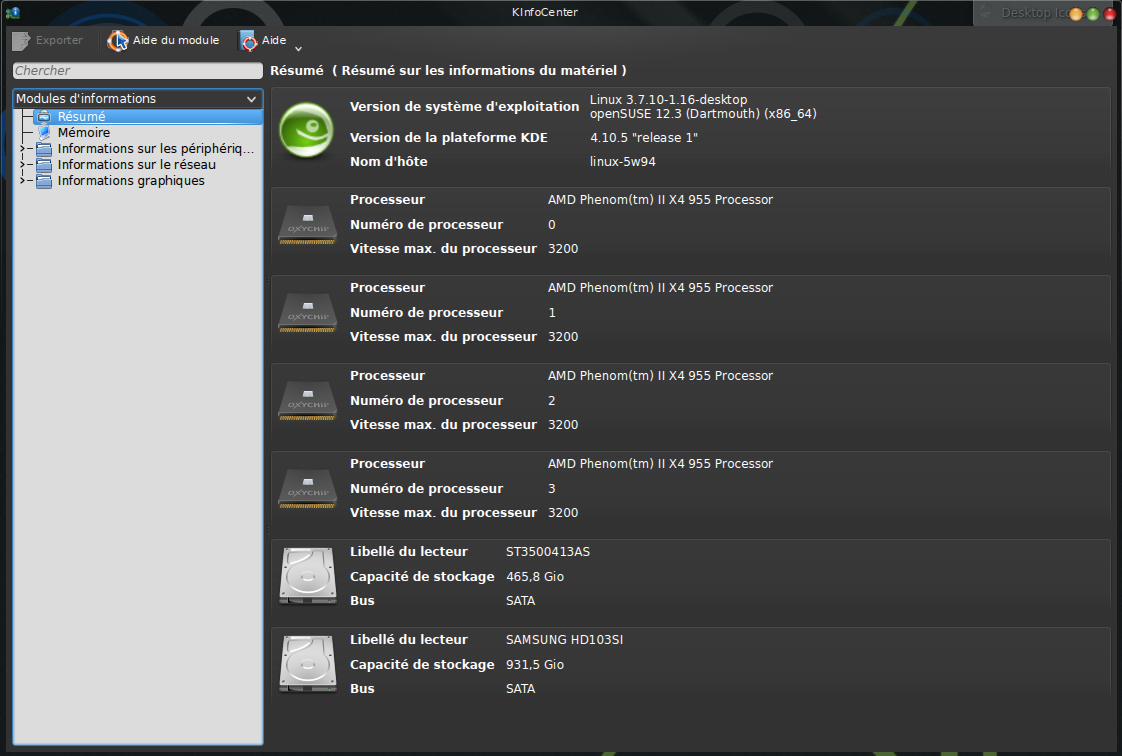
\includegraphics[width=\linewidth]{annexes/question4/systeme_1.png}

Mémoire\\
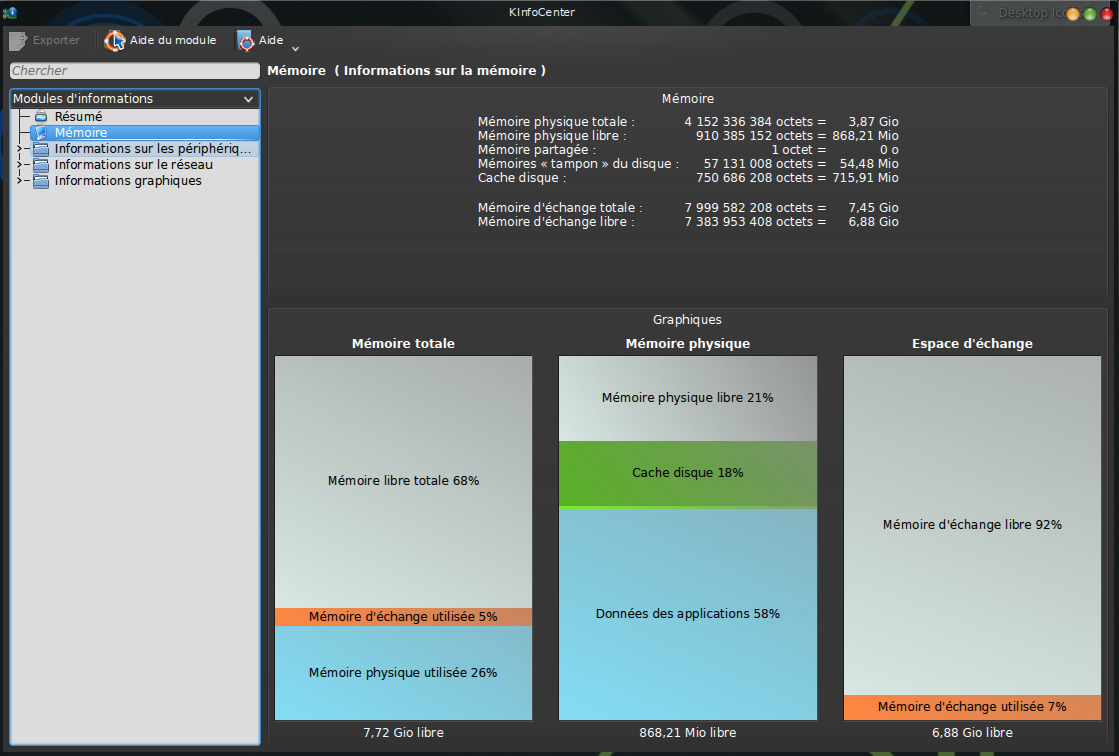
\includegraphics[width=\linewidth]{annexes/question4/systeme_2.png}

\subsection{Log de l'exécution de clustalw2.}\label{17}
\begin{verbatim}
 CLUSTAL 2.1 Multiple Sequence Alignments


Sequence format is Pearson
Sequence 1: lcl|XM_518463.3_cdsid_XP_518463.2        2058 bp
Sequence 2: lcl|XM_003833312.1_cdsid_XP_003833360.1  2004 bp
Sequence 3: lcl|XM_004043991.1_cdsid_XP_004044039.1  2004 bp
Sequence 4: lcl|XM_002816867.2_cdsid_XP_002816913.1  2043 bp
Sequence 5: lcl|XM_003266293.1_cdsid_XP_003266341.1  2004 bp
Sequence 6: lcl|XM_005553053.1_cdsid_XP_005553110.1  2004 bp
Sequence 7: lcl|NM_001266091.1_cdsid_NP_001253020.1  2043 bp
Sequence 8: lcl|XM_003922988.1_cdsid_XP_003923037.1  2004 bp
Start of Pairwise alignments
Aligning...

Sequences (1:2) Aligned. Score:  98
Sequences (1:3) Aligned. Score:  97
Sequences (1:4) Aligned. Score:  97
Sequences (1:5) Aligned. Score:  97
Sequences (1:6) Aligned. Score:  96
Sequences (1:7) Aligned. Score:  96
Sequences (1:8) Aligned. Score:  96
Sequences (2:3) Aligned. Score:  99
Sequences (2:4) Aligned. Score:  98
Sequences (2:5) Aligned. Score:  98
Sequences (2:6) Aligned. Score:  97
Sequences (2:7) Aligned. Score:  97
Sequences (2:8) Aligned. Score:  97
Sequences (3:4) Aligned. Score:  98
Sequences (3:5) Aligned. Score:  98
Sequences (3:6) Aligned. Score:  98
Sequences (3:7) Aligned. Score:  97
Sequences (3:8) Aligned. Score:  96
Sequences (4:5) Aligned. Score:  98
Sequences (4:6) Aligned. Score:  98
Sequences (4:7) Aligned. Score:  98
Sequences (4:8) Aligned. Score:  97
Sequences (5:6) Aligned. Score:  98
Sequences (5:7) Aligned. Score:  98
Sequences (5:8) Aligned. Score:  96
Sequences (6:7) Aligned. Score:  99
Sequences (6:8) Aligned. Score:  96
Sequences (7:8) Aligned. Score:  96
Guide tree file created:   [foxp4_ortho.dnd]

There are 7 groups
Start of Multiple Alignment

Aligning...
Group 1: Sequences:   2      Score:37737
Group 2: Sequences:   2      Score:37091
Group 3: Sequences:   3      Score:37148
Group 4: Sequences:   4      Score:37047
Group 5: Sequences:   5      Score:37481
Group 6: Sequences:   7      Score:37220
Group 7: Sequences:   8      Score:36779
Alignment Score 440506

CLUSTAL-Alignment file created  [foxp4_ortho.aln]
\end{verbatim}

\subsection{Log du travail de RepeatMasker sur le fichier foxp4\_ortho.fa.}\label{18}
\begin{verbatim}
There were no repetitive sequences detected in /usr/local/rmserver/tmp/RM2_foxp4_ortho.fa_1383262617
\end{verbatim}

\subsection{Log de l'exécution de Mavid sur foxp4\_ortho.fa.}\label{19}
\begin{verbatim}
./utils/randtree/randtree foxp4_ortho.fa
./mavid ./mavid.ph foxp4_ortho.fa

*******************************************************
*                                                     *
*                  Welcome to MAVID.                  *
*                  (version 2.0, build 4)             *
*                                                     *
*******************************************************


Aligning 1 versus 1
Aligning [0,2003] to [0,2057]
Aligning 1 versus 2
Aligning [0,2003] to [0,2058]
Aligning 1 versus 1
Aligning [0,2003] to [0,2042]
Aligning 1 versus 1
Aligning [0,2003] to [0,2003]
Aligning 1 versus 2
Aligning [0,2042] to [0,2003]
Aligning 2 versus 3
Aligning [0,2042] to [0,2042]
Aligning 3 versus 5
Aligning [0,2058] to [0,2042]
MAVID worked!

clustalw2 ./mavid.mfa -tree



 CLUSTAL 2.1 Multiple Sequence Alignments


Sequence format is Pearson
Sequence 1: lcl|XM_004043991.1_cdsid_XP_004044039.1  2059 bp
Sequence 2: lcl|XM_005553053.1_cdsid_XP_005553110.1  2059 bp
Sequence 3: lcl|XM_518463.3_cdsid_XP_518463.2        2059 bp
Sequence 4: lcl|XM_003266293.1_cdsid_XP_003266341.1  2059 bp
Sequence 5: lcl|NM_001266091.1_cdsid_NP_001253020.1  2059 bp
Sequence 6: lcl|XM_002816867.2_cdsid_XP_002816913.1  2059 bp
Sequence 7: lcl|XM_003833312.1_cdsid_XP_003833360.1  2059 bp
Sequence 8: lcl|XM_003922988.1_cdsid_XP_003923037.1  2059 bp

Phylogenetic tree file created:   [./mavid.ph]

../utils/root_tree/root_tree ./mavid.ph
./mavid ./mavid.ph foxp4_ortho.fa

*******************************************************
*                                                     *
*                  Welcome to MAVID.                  *
*                  (version 2.0, build 4)             *
*                                                     *
*******************************************************


Aligning 1 versus 1
Aligning [0,2003] to [0,2042]
Aligning 1 versus 1
Aligning [0,2057] to [0,2003]
Aligning 1 versus 2
Aligning [0,2003] to [0,2003]
Aligning 3 versus 1
Aligning [0,2003] to [0,2042]
Aligning 1 versus 4
Aligning [0,2003] to [0,2042]
Aligning 2 versus 5
Aligning [0,2042] to [0,2042]
Aligning 1 versus 7
Aligning [0,2003] to [0,2042]
MAVID worked!

clustalw2 ./mavid.mfa -tree



 CLUSTAL 2.1 Multiple Sequence Alignments


Sequence format is Pearson
Sequence 1: lcl|XM_003922988.1_cdsid_XP_003923037.1  2098 bp
Sequence 2: lcl|XM_005553053.1_cdsid_XP_005553110.1  2098 bp
Sequence 3: lcl|NM_001266091.1_cdsid_NP_001253020.1  2098 bp
Sequence 4: lcl|XM_003266293.1_cdsid_XP_003266341.1  2098 bp
Sequence 5: lcl|XM_004043991.1_cdsid_XP_004044039.1  2098 bp
Sequence 6: lcl|XM_518463.3_cdsid_XP_518463.2        2098 bp
Sequence 7: lcl|XM_003833312.1_cdsid_XP_003833360.1  2098 bp
Sequence 8: lcl|XM_002816867.2_cdsid_XP_002816913.1  2098 bp

Phylogenetic tree file created:   [./mavid.ph]

../utils/root_tree/root_tree ./mavid.ph
\end{verbatim}

\subsection{Arbre phylogénique créé par ClustalW}\label{20}
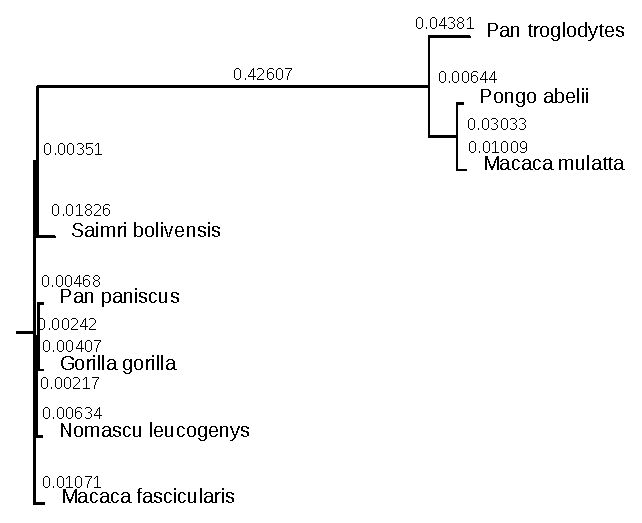
\includegraphics{annexes/q4_cds/clustalw/foxp4_ortho.eps}

\subsection{Arbre phylogénique créé par Dialign}\label{21}
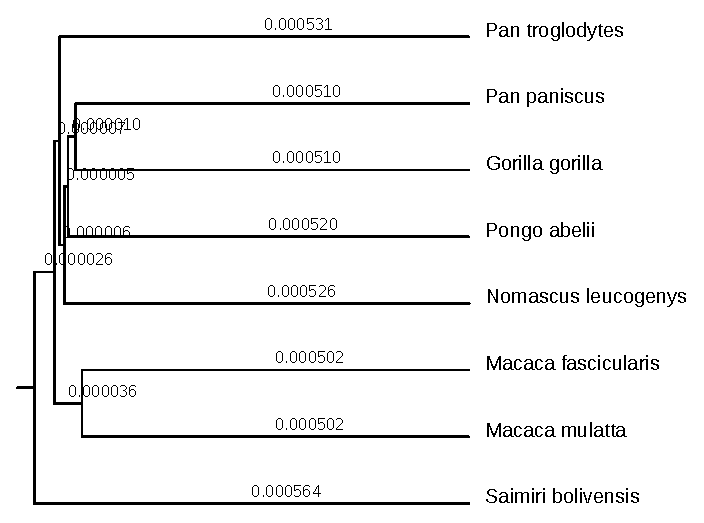
\includegraphics{annexes/q4_cds/dialign/foxp4_ortho.eps}

\subsection{Arbre phylogénique créé par Mavid}\label{22}
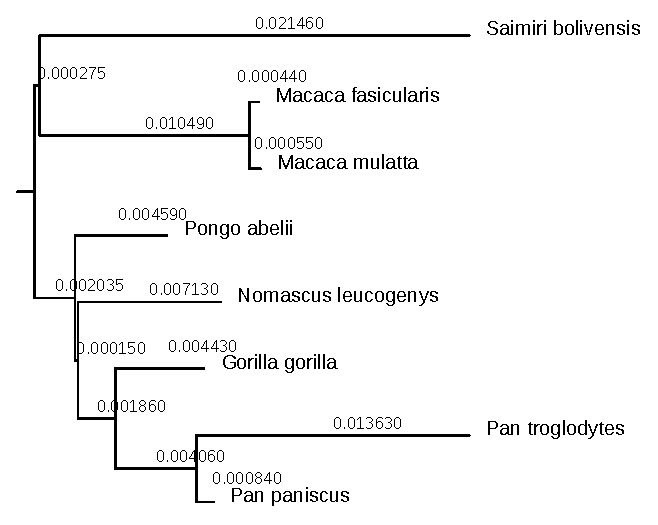
\includegraphics{annexes/q4_cds/Mavid/mavid.eps}

\subsection{Script biopython pour identifier la composition du vecteur pANNE}\label{23}
\begin{lstlisting}[frame=single,numbers=left,language=Python]
# *- coding:utf-8 -* #

# Script pour le numéro 3 du devoir 1: Cette partie ne fait
#qu'envoyer la requête blast au serveur du NCBI, et ensuite
#enregistre le résultat dans un fichier.

from Bio.Blast import NCBIWWW
from Bio.Blast import NCBIXML

path_fichier = "annexes/question_3/"
nom_resultat = "blast_fichier"
LEN_THRESH = 100
E_THRESH = 1e-50
# Tout d'abord on ouvre le fichier

sequence = ""
with open(path_fichier+"pANNE.txt", 'r') as f:
    for line in f:
        sequence = sequence + line.strip()

#On enlève les retour de chariot du fichier
i = 1
while len(sequence) > LEN_THRESH:

#Maintenant, on fait le blast
    print "i = " + str(i)
    print "on fait un blast sur la séquence de longeur " 
      + str(len(sequence))
    result_handle = NCBIWWW.qblast("blastn", "nr", 
      sequence, megablast=True)

#on enregistre le résultat
    save_file = open(path_fichier+nom_resultat+str(i)+".xml", "w")
    save_file.write(result_handle.read())
    save_file.close()
    result_handle.close()

    list_start = []
    list_end = []
    sequences = []
#Maintenant on enlève de la séquence les zones identifiées
    with open(path_fichier+nom_resultat+str(i)+".xml", "r") as result:
        blast_record = NCBIXML.read(result)
        alignment = blast_record.alignments[0]
        for alignment in blast_record.alignments:
            for hsp in alignment.hsps:
#On met à jour la séquence pour enlever ce résultat
                if hsp.expect < E_THRESH:
                    list_start.append(hsp.query_start)
                    list_end.append(hsp.query_end)
                
            break
#On a les points à enlever
#sort sur les listes
        list_start.sort()
        list_end.sort()
        start= -1
        end = -1
        for s_start, s_end in zip(list_start, list_end):
            if end < 0:
                sequences.append(sequence[: s_start-1])
                end = s_start-1
            else:
                end = s_start-1
                sequences.append(sequence[start: end])
            start = s_end -1
        sequences.append(sequence[start:])
        sequence = ""
        for fragment in sequences:
            sequence +=fragment
#Pour vérifier les résutats, j'enregistre la nouvelle 
#séquence dans un fichier
        print "On écrit le reste de la séquence avec i = " + str(i)
        with open(path_fichier+"pANNE"+str(i)+".txt", "w") as f:
            f.write(sequence)
    i +=1
\end{lstlisting}

\subsection{Temps d'exécution des alignements multiples}\label{24}
\begin{tabular}{|c|c|}
 \hline
 Programme & Temps d'exécution \\
 \hline
 ClustalW & real 0m4.840s \\
 \hline
 dialign & real 0m18.424s \\
 \hline
 Mavid & real 0m0.296s\\
 \hline
\end{tabular}

\subsection{Fichiers genbank utilisés pour ce rapport}\label{25}

 \footnotesize{
\begin{longtable}{|p{4.5cm}|p{3.5cm}|p{4.5cm}|p{3.5cm}|}
\hline
 Nom & Numéro d'accession & Nom & Numéro d'accession\\
 \hline \endhead
 Cloning Vector EN.Cherry, complete sequence & HM771696.1 & PGeneClip hMGFP Vector, complete sequence & AY744386.1 \\
 \hline
 Expression vector pHT2, complete sequence & AY773970.1 & Homo sapiens chromosome 6, GRCh37.p13 Primary Assembly & NC\_000006.11 \\
 \hline 
 SARS coronavirus MA15 ExoN1 isolate d3om5, complete genome & JF292906.1 & SARS coronavirus MA15 isolate d2ym4, complete genome & JF292909.1 \\
 \hline
  SARS coronavirus MA15 isolate d4ym5, complete genome & JF292915.1 & SARS coronavirus HKU-39849 isolate recSARS-CoV HKU-39849, 
  complete genome & JN854286 .1 \\
 \hline
   SARS coronavirus HKU-39849 isolate UOB, complete genome & JQ316196.1 & SARS coronavirus isolate Tor2/FP1-10912, complete genome & JX163923.1 \\
 \hline
 SARS coronavirus isolate Tor2/FP1-10851, complete genome & JX163924.1  & SARS coronavirus isolate Tor2/FP1-10895, complete genome & JX163925.1 \\
 \hline
  SARS coronavirus isolate Tor2/FP1-10912, complete genome & JX163926.1  & SARS coronavirus isolate Tor2/FP1-10851, complete genome & JX163927.1 \\
 \hline
   SARS coronavirus isolate Tor2/FP1-10895, complete genome & JX163928.1  & SARS coronavirus SinP3, complete genome & AY559090.1 \\
 \hline
  SARS coronavirus HKU-39849 isolate TCVSP-HARROD-00001, complete genome & GU553363.1  & SARS coronavirus HKU-39849 isolate recSARS-CoV HKU-39849, complete genome & JN854286.1 \\
 \hline
  SARS coronavirus HKU-39849 isolate TCVSP-HARROD-00002, complete genome & GU553364.1  & SARS coronavirus HKU-39849 isolate TCVSP-HARROD-00003, complete genome & GU553365.1 \\
 \hline
  SARS coronavirus Sin850, complete genome & AY559096.1  & SARS coronavirus MA15 isolate P3pp3, complete genome & FJ882948.1 \\
 \hline
  SARS coronavirus MA15 ExoN1 isolate P3pp3, complete genome & FJ882951.1  & SARS coronavirus MA15 isolate P3pp4, complete genome & FJ882952.1 \\
 \hline
  SARS coronavirus MA15, complete genome & FJ882957.1   & SARS coronavirus MA15 isolate P3pp7, complete genome & FJ882958.1 \\
 \hline
  SARS coronavirus MA15 ExoN1 isolate P3pp6, complete genome & FJ882959.1   & SARS coronavirus MA15 isolate P3pp5, complete genome & FJ882961.1 \\
 \hline
   SARS coronavirus ExoN1 isolate c5P1, complete genome & JF292922.1   & SARS coronavirus ExoN1 isolate c5P10, complete genome & JX162087.1 \\
 \hline
 SARS coronavirus ExoN1 strain & KF514407.1   &  PREDICTED: Pan troglodytes forkhead box P4, transcript variant 2 (FOXP4), mRNA & XM\_518463.3  \\
 \hline
  PREDICTED: Pan paniscus forkhead box P4, transcript variant 2 (FOXP4), mRNA. & XM\_003833312.1 & PPREDICTED: Gorilla gorilla gorilla forkhead box P4, transcript variant 2 (FOXP4), mRNA. & XM\_004043991.1  \\
 \hline
   PREDICTED: Pongo abelii forkhead box P4, transcript variant 1 (FOXP4), mRNA. & XM\_002816867.2 & PREDICTED: Nomascus leucogenys forkhead box P4, transcript variant 2 (FOXP4), mRNA. & XM\_003266293.1  \\
 \hline
  PREDICTED: Macaca fascicularis forkhead box P4 (FOXP4), transcript variant X3, mRNA. & XM\_005553053.1 & Macaca mulatta forkhead box P4 (FOXP4), mRNA. & NM\_001266091.1  \\
 \hline
   PREDICTED: Saimiri boliviensis boliviensis forkhead box P4, transcript variant 2 (FOXP4), mRNA & XM\_003922988.1 &  Homo sapiens chromosome 2, GRCh37.p13 Primary Assembly &  NC\_000002.11 \\
 \hline
   Homo sapiens amyotrophic lateral sclerosis 2 (juvenile) (ALS2), transcript variant 1, mRNA & NM\_020919.3 &  Homo sapiens amyotrophic lateral sclerosis 2 (juvenile) (ALS2), transcript variant 2, mRNA &  NM\_001135745.1 \\
 \hline
  Pan troglodytes chromosome 2B, Pan\_troglodytes-2.1.4 & NC\_006470.3 &  Macaca mulatta chromosome 12, Mmul\_051212, whole genome shotgun sequence &  NC\_007869.1 \\
 \hline
   Canis lupus familiaris breed boxer chromosome 37, CanFam3.1, whole genome shotgun sequence & NC\_006619.3 &  Bos taurus breed Hereford chromosome 2, Bos\_taurus\_UMD\_3.1, whole genome shotgun sequence &  AC\_000159.1 \\
 \hline
    Mus musculus strain C57BL/6J chromosome 1, GRCm38.p1 C57BL/6J & NC\_000067.6 &  Rattus norvegicus strain BN/SsNHsdMCW chromosome 9, Rnor\_5.0 &  NC\_005108.3 \\
 \hline
  Gallus gallus isolate \#256 breed Red Jungle fowl, inbred line UCD001 chromosome 7, Gallus\_gallus-4.0, whole genome shotgun sequence & NC\_006094.3 &  Danio rerio strain Tuebingen chromosome 6, Zv9 &  NC\_007117.5 \\
 \hline
 Homo sapiens chromosome 2 genomic contig, GRCh37.p13 Primary Assembly & NT\_005403.17 &  & \\
 \hline
\end{longtable}
}
\endgroup

%
%Bibiographie
%
\begin{thebibliography}{99}
{\small
\bibitem{UCSC genome browser}
    Kent WJ, Sugnet CW, Furey TS, Roskin KM, Pringle TH, Zahler AM, Haussler D. The human genome browser at UCSC. 
    \emph{Genome Res.} 2002 Jun;12(6):996-1006. 
\bibitem{Genetics Home Reference}
    National Library of Medicine (US). Genetics Home Reference [Internet]. Bethesda (MD): The Library; 2013 Oct 26. ALS2; [reviewed 2012
    Aug; cited 2013 Oct 26]. Available from: http://ghr.nlm.nih.gov/gene/ALS2
\bibitem{Wikipedia-SAL}
  Sclérose latérale amyotrophique. In Wikipedia. Retrieved October 26, 2013, from
  \url{http://fr.wikipedia.org/wiki/Sclerose_laterale_amyotrophique}
\bibitem{MPP4}
  Stohr, H., Weber, B. H. F. Cloning and characterization of the human retina-specific gene MPP4, a novel member of the p55 subfamily of
  MAGUK proteins. Genomics 74: 377-384, 2001. [PubMed: 11414766] [Full Text: Elsevier Science]
\bibitem{Wikipedia-pseudo}
  Pseudogène. In Wikipedia. Retrieved October 26, 2013, from \url{http://fr.wikipedia.org/wiki/Pseudogene}
\bibitem{TMEM237}
  Huang, L., Szymanska, K., Jensen, V. L., Janecke, A. R., Innes, A. M., Davis, E. E., Frosk, P., Li, C., Willer, J. R., Chodirker, 
  B. N.,  Greenberg, C. R., McLeod, D. R., and 31 others. TMEM237 is mutated in individuals with a Joubert syndrome related disorder
  and expands
  the role of the TMEM family at the ciliary transition zone. Am. J. Hum. Genet. 89: 713-730, 2011. [PubMed: 22152675] [Full Text:
  Elsevier Science]
\bibitem{OMIM-PLS}
  Online Mendelian Inheritance in Man, OMIM®. Johns Hopkins University, Baltimore, MD. MIM Number: 606353: 03/26/2009: . 
  World Wide Web URL: http://omim.org/
\bibitem{OMIM-ALS}
  Online Mendelian Inheritance in Man, OMIM®. Johns Hopkins University, Baltimore, MD. MIM Number: 205100: 07/19/2012: . 
  World Wide Web URL: http://omim.org/
\bibitem{OMIM-IAHSP}
  Online Mendelian Inheritance in Man, OMIM®. Johns Hopkins University, Baltimore, MD. MIM Number: 607225: 09/17/2013: . 
  World Wide Web URL: http://omim.org/
\bibitem{IAHSP}
  Eymard-Pierre, E., Lesca, G., Dollet, S., Santorelli, F. M., di Capua, M., Bertini, E., Boespflug-Tanguy, O. Infantile-onset ascending
  hereditary spastic paralysis is associated with mutations in the alsin gene. Am. J. Hum. Genet. 71: 518-527, 2002. [PubMed: 12145748,
  images] [Full Text: Elsevier Science]
\bibitem{OMIM-IAHSP}
  Online Mendelian Inheritance in Man, OMIM®. Johns Hopkins University, Baltimore, MD. MIM Number: 606352: 09/16/2013: . 
  World Wide Web URL: http://omim.org/
\bibitem{Yang and al.}
  Yang, Y., Hentati, A., Deng, H.-X., Dabbagh, O., Sasaki, T., Hirano, M., Hung, W.-Y., Ouahchi, K., Yan, J., Azim, A. C., Cole, N.,
  Gascon, G., Yagmour, A., Ben-Hamida, M., Pericak-Vance, M., Hentati, F., Siddique, T. The gene encoding alsin, a protein with three
  guanine-nucleotide exchange factor domains, is mutated in a form of recessive amyotrophic lateral sclerosis. Nature Genet. 29: 160-165,
  2001. Note: Erratum: Nature Genet. 29: 352 only, 2001. [PubMed: 11586297] [Full Text: Nature Publishing Group]
\bibitem{Hadano and al.}
  Hadano, S., Hand, C. K., Osuga, H., Yanagisawa, Y., Otomo, A., Devon, R. S., Miyamoto, N., Showguchi-Miyata, J., Okada, Y., Singaraja,
  R., Figlewicz, D. A., Kwiatkowski, T., and 9 others. A gene encoding a putative GTPase regulator is mutated in familial amyotrophic
  lateral sclerosis 2. Nature Genet. 29: 166-173, 2001. Note: Erratum: Nature Genet. 29: 352 only, 2001. [PubMed: 11586298] [Full Text:
  Nature Publishing Group]
\bibitem{CAP3}
  Huang, X. and Madan, A. (1999) CAP3: A DNA Sequence Assembly Program. Genome Research, 9: 868-877.
\bibitem{BLAST}
  Basic Local Alignment Search Tool (Altschul et al., J Mol Biol 215:403-410; 1990).
\bibitem{CLUSTALW}
  ClustalW and ClustalX version 2 (2007) Larkin MA, Blackshields G, Brown NP, Chenna R, McGettigan PA, McWilliam H, Valentin F, 
  Wallace IM, Wilm A, Lopez R, Thompson JD, Gibson TJ and Higgins DG Bioinformatics 2007 23(21): 2947-2948.
  doi:10.1093/bioinformatics/btm404 
\bibitem{DIALIGN}
  A.R. Subramanian, M. Kaufmann, B. Morgenstern (2008)
  DIALIGN-TX: greedy and progressive approaches for segment-based multiple sequence alignment.
  Algorithms for Molecular Biology 3,6.
\bibitem{RepeatMasker}
 A.F.A. Smit, R. Hubley \& P. Green, unpublished data. Current Version: open-4.0.3 ( RMLib: 20130422 \& Dfam: 1.2 )
\bibitem{Mower et Annaiah}
  Mower, Jeff, Annaiah, Kiran.Multiple Sequence Alignment. A survey of the various programs available and application of MSA in
  addressing certain biological problems. PowerPoint Presentation. School of Informatics, Indiana University. Downloaded on
  2013-10-31. Available at bio.informatics.indiana.edu/L529/papers/kiran-jeff.ppt.
}
\end{thebibliography}

\end{document}